\documentclass[12pt]{report}

\usepackage[utf8]{inputenc}
\usepackage[T1]{fontenc}
\usepackage{natbib}
\usepackage[frenchb]{babel}

\usepackage{amsmath}
\usepackage{stmaryrd}
\usepackage{bm}

\usepackage[dvipsnames]{xcolor}
\definecolor{DarkGray}{gray}{0.35}

\usepackage{listings}
\definecolor{darkWhite}{gray}{0.93}
\definecolor{gray}{gray}{0.5}
\definecolor{green}{RGB}{0, 153, 51}
\definecolor{orange}{RGB}{255,127,0}
\lstset{
aboveskip=3mm,
belowskip=-2mm,
backgroundcolor=\color{darkWhite},
basicstyle=\footnotesize,
breakatwhitespace=false,
breaklines=true,
captionpos=b,
commentstyle=\color{green},
deletekeywords={...},
escapeinside={\%*}{*)},
extendedchars=true,
framexleftmargin=16pt,
framextopmargin=3pt,
framexbottommargin=6pt,
frame=tb,
keepspaces=true,
keywordstyle=\color{blue},
morekeywords={*,...},
numbers=left,
numbersep=10pt,
numberstyle=\tiny\color{gray},
rulecolor=\color{black},
showspaces=false,
showstringspaces=false,
showtabs=false,
stepnumber=1,
stringstyle=\color{orange},
tabsize=4,
title=\lstname,
}

\usepackage{graphicx}
\graphicspath{{pictures/}}

\usepackage{forest}

\usepackage[left=2cm,right=2cm,top=2cm,bottom=2cm]{geometry}

\usepackage{ifthen}
\usepackage{ifpdf}
\ifpdf
\usepackage[pdftex]{hyperref}
\else
\usepackage{hyperref}
\fi

\title{Propagation de la lumière dans un milieu participant de type fumée}
\author{Elsa Tamisier}
\date{Vendredi 6 juillet 2018}


\begin{document}

%%%%%%%%%%%%%%%%%%
%%% First page %%%
%%%%%%%%%%%%%%%%%%

\begin{titlepage}
\begin{center}


{\large \textbf{\textsc{Université de Poitiers}}}\\[0.5cm]

\vspace{6cm}

% Title
\rule{\linewidth}{0.5mm} \\[0.4cm]
{ \LARGE \bfseries Propagation de la lumière dans un milieu participant de type fumée \\[0.4cm] }
\rule{\linewidth}{0.5mm} \\[1.5cm]

% Author and supervisor
\noindent
\begin{minipage}[t][0.4cm]{0.9\textwidth}
  \begin{flushleft} \large
    \emph{\textbf{Auteur}}\\
    Elsa \textsc{Tamisier}
  \end{flushleft}
\end{minipage}%

\begin{minipage}{0.9\textwidth}
  \begin{flushright} \large
        \emph{\textbf{Encadrants}} \\
        Lilian \textsc{Aveneau}\\
        Pierre \textsc{Combeau}\\
    \end{flushright}
\end{minipage}

\vspace{5cm}

\includegraphics[width=60mm]{xlim_logo.png}\\

\vfill

% Bottom of the page
{\textsc{06 Juillet 2018}}

\end{center}
\end{titlepage}


%%%%%%%%%%%%%%%%%%%%%%%%%%%%%
%%% Non-significant pages %%%
%%%%%%%%%%%%%%%%%%%%%%%%%%%%%

\renewcommand*\contentsname{\textsc{Sommaire}}

\tableofcontents


%%%%%%%%%%%%%%%%%%%%%%%%%%%%%%%%%%%%%%%%%%%%
%%% Content of the report and references %%%
%%%%%%%%%%%%%%%%%%%%%%%%%%%%%%%%%%%%%%%%%%%%

\chapter*{Introduction}
\addcontentsline{toc}{chapter}{Introduction}

En informatique graphique, et plus précisément dans le domaine du rendu, il est courant de trouver des recherches, expérimentations, démonstrations, ... sur la façon dont la lumière va être rendue. La lumière a toujours intéressé les savants et il existe de nombreux papiers et manuscrits traitant de ce sujet. Physiquement (et très basiquement résumé), la lumière est l'énergie transportée par les \textit{photons}, qui se déplacent selon une onde. Cette onde n'a pas toujours la même longueur $\lambda$ et c'est cette différence qui produit un large spectre de lumière.\par
Ces photons interagissent avec toutes les particules qu'ils vont croiser. Certaines interactions sont extrêmement faibles, c'est par exemple le cas de l'air qui ne modifie pas (sur une distance pas trop importante) notre perception des couleurs. D'autres à l'inverse vont avoir un impact plus important, telles les interactions dues au passage de la lumière dans de la fumée.\newline\par

Ce rapport résume ce que j'ai pu lire et comprendre autour de la propagation de la lumière dans un milieu participant, afin de proposer un algorithme simple permettant de calculer la radiance d'un rayon récupérée à la sortie d'un milieu participant (plus précisément de la fumée).\newline\par

Dans un premier temps je présente rapidement la méthode de Monte Carlo qui permet d'algorithmiquement approcher une intégrale sur un domaine donné, en utilisant l'aléatoire et les probabilités. Je ne m'attarde ni sur les démonstrations ni sur les optimisations que je ne compte pas appliquer pour le moment.\par
Puis je présente l'équation du transfert de la lumière (et plus précisément l'équation en potentiel) qui sera la base de notre démarche future.\par
Ensuite se trouve un court résumé expliquant ce que sont les fonctions de phase puis quelques fonctions de phase usuelles.\par
Le troisième chapitre se penche sur les différentes interactions qui s'appliquent sur la radiance d'un rayon lorsque celui-ci passe dans un milieu participant.\par
Dans le dernier chapitre, qui est très court, est introduite l'équation de transfert, qui combine l'ensemble des interactions. C'est avec cette équation de transfert et l'équation du transport de la lumière qu'il me faudra réfléchir à une solution.\par
\chapter{Monte Carlo}

\section{La méthode}

La méthode de Monte Carlo permet de trouver l'approximation d'une intégrale grâce à un échantillonnage aléatoire sur le domaine d'intégration. Soit $I$ une intégrale sur son domaine $\Omega$ :
\large \begin{equation}
    I = \int_{\Omega}f(x)dx
.\end{equation} \normalsize \par
Prenons un échantillon de N variable aléatoires $x_{i}$ avec leur probabilités d'échantillonnage $p(x_{i})$. Alors nous avons une approximation de l'intégrale avec $\hat I$, l'\textbf{estimateur} de Monte Carlo :
\large \begin{equation}
    \hat I = \frac{1}{N}\sum\limits_{i=1}^{N} \frac{f(x_{i})}{p(x_{i})}
.\end{equation} \normalsize \par
$p(x_{i})$ est appelée la \textit{pdf} (Probability Density Function) de $x_{i}$. Nous avons les conditions suivantes sur une pdf :
\large \begin{equation}
    \forall x \in \Omega
    \text{,}\quad
    p(x) \geq 0
    \quad\text{et}\quad
    \int_{\Omega}p(x)dx=1
.\end{equation} \normalsize \newline\par

$\hat I$ n'est qu'une approximation de $I$. Puisque nous travaillions avec un échantillon aléatoire, il est possible d'en tirer un nouveau et d'obtenir une nouvelle approximation. Aussi, il suffit de calculer plusieurs estimations et d'en faire la moyenne pour s'approcher de plus en plus de la valeur de $I$. L'estimateur $\hat I$ de Monte Carlo converge vers $I$ :
\large \begin{equation}
    E\left[\hat I\right] = I
.\end{equation} \normalsize \newline\par

Après des calculs basiques de probabilités, il est facile de trouver l'écart-type de $\hat I$ :
\large \begin{equation}
    \sigma\left[\hat I\right] = \frac{1}{\sqrt{N}}\sigma\left[\frac{f(x)}{p(x)}\right]
.\end{equation} \normalsize \par
Ceci indique que l'erreur diminue avec l'augmentation de la racine carré de la taille de l'échantillonnage. C'est-à-dire que pour diviser l'erreur par 2, il faut multiplier le nombre d'échantillons par 4. Cette erreur n'est pas dépendante de la dimension du domaine d'intégration, ce qui est un avantage principal de la méthode de Monte Carlo.


\section{L'échantillonnage}

En informatique il est courant de générer des variables pseudo-aléatoires selon une loi uniforme sur $[0, 1]$. De nombreux algorithmes plus ou moins robustes permettent de tirer des séquences de nombres qui passeront les tests d'aléatoire.\par
Cependant, comme nous l'avons vu précédemment, la méthode de Monte Carlo utilise des variable aléatoires distribuées selon une loi de densité $p(x)$, qui est propre au domaine d'intégration. Il nous faut donc pouvoir générer de tels échantillons, en partant de variables aléatoires uniformes.

\subsection{Méthode d'inversion}

La première méthode, la plus efficace si la \textit{pdf} le permet, est la méthode d'inversion. Celle-ci se base sur le calcul de la CDF (Cumulative Distribution Function) puis son inversement.\par
La \textit{CDF} $P(x)$ associée à la \textit{pdf} $p(x)$ est :
\large \begin{align}
    P(x) &= p(y \in \Omega, y \geq x) .\\
         &= \int_{-\infty}^{x} p(y) dy
.\end{align} \normalsize \newline\par

A partir de cette \textit{CDF} et d'une variable aléatoire uniforme $\xi_{i}$, nous pouvons générer une variable aléatoire $x_{i}$ selon la \textit{pdf} avec la relation suivante :
\large \begin{equation}
    x_{i} = P^{-1}(\xi_{i})
.\end{equation} \normalsize \par
Il suffit donc de réaliser $N$ fois ce calcul à partir d'un échantillon uniforme de taille $N$, et nous aurons notre échantillon suivant la densité $p(x)$.

\subsection{Méthode de rejet}

Cependant une \textit{pdf} ne permet pas toujours facilement de trouver la \textit{CDF} associée. Ou bien cette dernière n'est pas toujours inversible (ou cette transformation est lourde à faire d'un point de vue algorithmique). Il existe donc une autre méthode pour produire un échantillonnage adéquat.\par
Pour cette méthode, il faut qu'en plus de notre densité $p(x)$ difficilement utilisable, nous ayons une densité $q(x)$ pour laquelle nous savons générer un échantillonnage (par exemple avec la méthode d'inversion), telle que :
\large \begin{equation}
    \forall x \in \Omega
    \text{,}\quad
    p(x) \leq c \times q(x)
.\end{equation} \normalsize
avec $c$ une constante positive choisie judicieusement (voir ci-après).\newline\par

Avec cette densité $q(x)$, il faut générer des échantillons $x_{i}$ et, pour chacun, vérifier que
\large \begin{equation}\label{eq:condition_rejet}
    \xi \times c \times q(x_{i}) \leq p(x_{i})
.\end{equation} \normalsize
où $\xi$ est une variable aléatoire qui suit une loi uniforme $U(0, 1)$.\par
Si la condition \ref{eq:condition_rejet} est vérifiée, alors $x_{i}$ est un échantillon accepté et sera utilisé. Sinon, une nouvelle paire $(x_{i}, \xi)$ est générée et testée à nouveau.\newline\par

Plus l'écart entre les deux densités $p(x)$ et $cq(x)$ est grand, plus il y a des chances que l'échantillon $x_{i}$ soit rejeté. Aussi, pour optimiser la vitesse de génération de l'échantillonnage, il faut chercher à prendre la constante $c$ la plus petite possible.


\subsection{Direction aléatoire en coordonnées sphériques}

Dans le cadre de la propagation de la lumière, nous aurons à échantillonner sur un hémisphère pour lancer le rayon, puis sur des sphères lorsque nous calculerons le comportement de la lumière sur une particule du milieu participant. L'échantillonnage d'une direction est donc plutôt à faire en coordonnées sphériques où elle est représentée par deux données $(\theta, \phi)$ qui représente un point sur la surface de la sphère. $\theta$ est appelé le \textit{zenith} (ou \textit{élévation}) du point. Et $\phi$ est appelé l'\textit{azimuth} du point.\par
Nous avons les intervalles de définition suivants :
\large \begin{equation*}
    \theta \in \left\{
        \begin{array}{ll}
            \left[ 0, \pi \right] & \text{sur une sphère} .\\
            \left[ 0, \frac{\pi}{2} \right] & \text{sur un hémisphère}.
        \end{array}
    \right.
\end{equation*}
\begin{equation*}
    \phi \in \left[ 0, 2\pi \right]
.\end{equation*} \normalsize \newline\par

Mais il ne suffit pas de tirer deux variables aléatoires uniformes sur l'intervalle correspondant pour générer un bon échantillon $(\theta, \phi)$. En effet, imaginons que l'on coupe des tranches de notre sphères, orthogonalement à l'axe de révolution de l'angle $\phi$. Alors, peu importe la valeur de $\theta$ et donc l'aire de notre cercle, $\phi$ sera distribué de la même manière. De manière uniforme, nous aurons donc autant d'échantillons sur un cercle large (lorsque $\theta$ est proche de $\frac{\pi}{2}$) que sur un cercle bien plus petit (lorsque $\theta$ est proche de $0$). il en découlera une mauvaise répartition des directions échantillonnées. Et l'échantillonnage ne sera plus uniforme sur la sphère.\newline\par

Il faut échantillonner la direction $\overrightarrow{\omega}$ selon la \textit{pdf} $p(\overrightarrow{\omega})$. C'est-à-dire qu'il faut échantillonner chacune des deux variables $\theta$ et $\phi$ selon leur \textit{pdf} respectives $p(\theta)$ et $p(\phi)$ associée à $p(\overrightarrow{\omega})$. Plus précisément, il ne faut pas échantillonner les deux variables indépendamment, mais en prenant en compte la valeur trouvée pour $\theta$ lorsque l'on va vouloir générer $\phi$.\par
Avec des calculs en partant de l'angle solide $d\overrightarrow{\omega}$ et en sachant que $p(\overrightarrow{\omega})$ est constante (puisque nous voulons une distribution uniforme sur la sphère ou l'hémisphère), nous arrivons aux fonctions suivantes.\newline\par
\textbf{Pour un hémisphère.}
\large \begin{equation}
    p(\overrightarrow{\omega}) = \frac{1}{2\pi}
.\end{equation}
\begin{align}
    &p(\theta) = sin(\theta) .\\
    &p(\phi \mid \theta) = \frac{1}{2\pi}
.\end{align}
\begin{align}
    &P(\theta) = 1 - cos\theta .\\
    &P(\phi \mid \theta) = \frac{\phi}{2\pi}
.\end{align}
\begin{align}
    &P^{-1}(\xi_{\theta}) = cos^{-1}(1 - \xi_{\theta}) .\\
    &P^{-1}(\xi_{\phi}) = 2 \pi \xi_{\phi}
.\end{align} \normalsize
où $\xi_{\theta}$ et $\xi_{\phi}$ sont des variables aléatoires suivant la loi uniforme.\newline\par

\textbf{Pour une sphère.}
\large
\begin{equation}
    p(\overrightarrow{\omega}) = \frac{1}{4\pi}
.\end{equation}
\begin{align}
    &p(\theta) = \frac{sin(\theta)}{2} \\
    &p(\phi \mid \theta) = \frac{1}{2\pi}
.\end{align}
\begin{align}
    &P(\theta) = \frac{1 - cos\theta}{2} .\\
    &P(\phi \mid \theta) = \frac{\phi}{2\pi}
.\end{align}
\begin{align}
    &P^{-1}(\xi_{\theta}) = cos^{-1}(1 - 2\xi_{\theta}) .\\
    &P^{-1}(\xi_{\phi}) = 2 \pi \xi_{\phi}
.\end{align} \normalsize
\chapter{LTE}

\section{Deux équations}

L'équation du transport de la lumière \textit{LTE} (Light Transport Equation) décrit la distribution de la radiance dans toute la scène. Elle permet de connaître la radiance réfléchie en un point d'une surface, en fonction de l'émission de cette surface, sa BRDF et toutes les autres surfaces de la scène pouvant venir perturber le rayon.\newline\par

Il existe deux LTE différentes : l'équation de \textit{rendu} et l'équation en \textit{potentiel}. Dans l'équation de rendu, les rayons étudiés partent du récepteur et on cherche des chemins remontant jusqu'aux sources. L'équation de potentiel partage le même principe mais dans l'autre sens, les rayons étant tiré de la source et on calcule leur contributions sur le récepteur.\par
Dans les deux cas, il s'agit de trouver l'éclairage global de la scène et non pas juste l'éclairage direct qui ne prend en compte que les rayons provenant directement d'une source de lumière. Ici, on souhaite également tenir compte de la radiance provenant de réflexions sur des surfaces n'étant pas forcément auto-émittante.\newline\par

L'\textbf{équation de rendu} s'exprime par la formule :
\large \begin{equation}\label{eq:LTE_rendu}
    L_r(x, \overrightarrow{\omega_r}, t) =
        L_e(x, \overrightarrow{\omega_r}, t) +
        \int_{\Omega_x}
            f_r(x, \overrightarrow{\omega_i} \longrightarrow \overrightarrow{\omega_r})
            L_i(x, \overrightarrow{\omega_i}, t)
            |\overrightarrow{\omega_i}, \overrightarrow{n} |
        d\overrightarrow{\omega_i}
,\end{equation} \normalsize
où $L_e(x, \overrightarrow{\omega_r}, t)$ est la lumière auto-émise par la surface, \\
$L_i(x, \overrightarrow{\omega_i}, t)$ est la radiance incidente dans la direction $\overrightarrow{\omega_i}$, \\
$\overrightarrow{n}$ est la normale à la surface au point $x$, \\
$f_r(x, \overrightarrow{\omega_i} \longrightarrow \overrightarrow{\omega_r})$ est la BRDF de la surface au point x dans le sens de propagation $\overrightarrow{\omega_i} \longrightarrow \overrightarrow{\omega_r}$.\newline\par

L'\textbf{équation en potentiel} s'exprime par la formule :
\large \begin{equation} \label{eq:LTE_potentiel}
    W(x, y, \overrightarrow{\omega_x}, t) =
        W_e(x, y, \overrightarrow{\omega_x}, t) +
        \int_{\Omega_z}
            f_r(z, \overrightarrow{\omega_x} \longrightarrow \overrightarrow{\omega_z})
            W(z, y, \overrightarrow{\omega_z}, t)
            |\overrightarrow{\omega_z}, \overrightarrow{n_z} |
        d\overrightarrow{\omega_z}
,\end{equation} \normalsize
où $W(x, y, \overrightarrow{\omega_x}, t)$ est l'action potentielle du point $x$ sur le point $y$ dans la direction $\overrightarrow{\omega_x}$, \\
$ W_e(x, y, \overrightarrow{\omega_x}, t)$ est l'action potentielle directe de la source au point $x$ sur le point $y$ suivant $\overrightarrow{\omega_x}$.\par
Dans ce rapport et pour ce qui suit, je me place dans le cas de l'équation en potentiel.

\section{Equation en potentiel avec réflexions}

L'éclairement reçu au niveau d'un récepteur positionné en $M_{rx}$ pour un rayonnement émis par une source positionnée en $M_{tx}$ est donné par :
\large \begin{equation}
    E(M_{tx}, M_{rx}, t) =
        \int_{\Omega_{tx}}
            L_e(M_{tx}, \overrightarrow{\omega_0}, t)
            W(M_{tx}, M_{rx}, \overrightarrow{\omega_0}, t)
            | \overrightarrow{\omega_0} \cdot \overrightarrow{n_{tx}} |
        d\overrightarrow{\omega_0}
,\end{equation} \normalsize
où $L_e(M_{tx}, \overrightarrow{\omega_0}, t)$ désigne le rayonnement sortant dans la direction $\overrightarrow{\omega_0}$.\newline\par

Cela dit, la plupart des rayons lancés de la source ne vont pas directement au récepteur et sont d'abord réfléchis par des surfaces. Aussi, après $k$ réflexions, nous avons l'équation suivante :
\large \begin{equation}
    E_k(M_{tx}, M_{rx}, t) =
        \int_{\Omega_{tx}} \cdots
            \int_{\Omega_k}
                f_k(\bar{x}, t)
            d\overrightarrow{\omega_0}
            \cdots
        d\overrightarrow{\omega_k}
,\end{equation} \normalsize
où $\bar{x}$ correspond au trajet de propagation de la lumière entre $M_{tx}$ et $M_{rx}$ rebondissant sur les $x_i$ points de réflexions ($i \in \llbracket1, k\rrbracket$). Et 
\large \begin{multline}
    f_k(\bar{x}, t) =
        | \overrightarrow{\omega_0} \cdot \overrightarrow{n_{tx}} |
        L_e(M_{tx}, \overrightarrow{\omega_0}, t)
        rect\left(
            \frac
                {| \overrightarrow{x_k M{rx}} \cdot \overrightarrow{n_{rx}} |}
                {cos(FOV) \Vert \overrightarrow{x_k M_{rx}}}
        \right)
        W_l(x_k, M_{rx}, \overrightarrow{\omega_k} t) \\
        \times
        \prod\limits_{i=1}^k
            f_r(x_i, \overrightarrow{\omega_{i-1}} \longrightarrow \overrightarrow{\omega_i})
            | \overrightarrow{\omega_i} \cdot \overrightarrow{n_i} |
,\end{multline} \normalsize
avec la fonction $rect$ qui vérifie que $x_k$ est dans le champ de vision du récepteur et $W_l(x_k, M_{rx}, t)$ qui est l'action potentielle directe du dernier point de réflexion $x_k$ sur le récepteur.

\section{Equation en potentiel optimisée}
\label{sec:LTE}

L'équation précédente permet seulement de suivre un chemin de $k$ réflexions puis de regarder l'action potentielle sur le récepteur du dernier point $x_k$ du chemin. De ce fait, les actions potentielles des points de réflexions $x_i$ ($1 \leq i < k$) doivent être calculés indépendemment les uns des autres, et nous aurons à lancer $k$ fois le même chemin (de plus en plus long) pour avoir les $k$ contributions.\newline\par

Une optimisation possible de l'équation cherche donc à ne pas répéter inutilement les réflexions. Elle consiste à calculer, pour chaque point $x_i$ son action potentielle sur le récepteur dès le premier lancé de rayon. Cette technique s'appelle l'\textit{estimation du prochain évènement} (NEE "Next Event Estimation"). Ces contributions sont représentées dans la figure \ref{fig:LTE_potentiel} par les traits en pointillés reliant un point de réflexion $x_i$ à un récepteur $M_{rx}$.\newline

\begin{figure}[h!]\label{fig:LTE_potentiel}
\centering
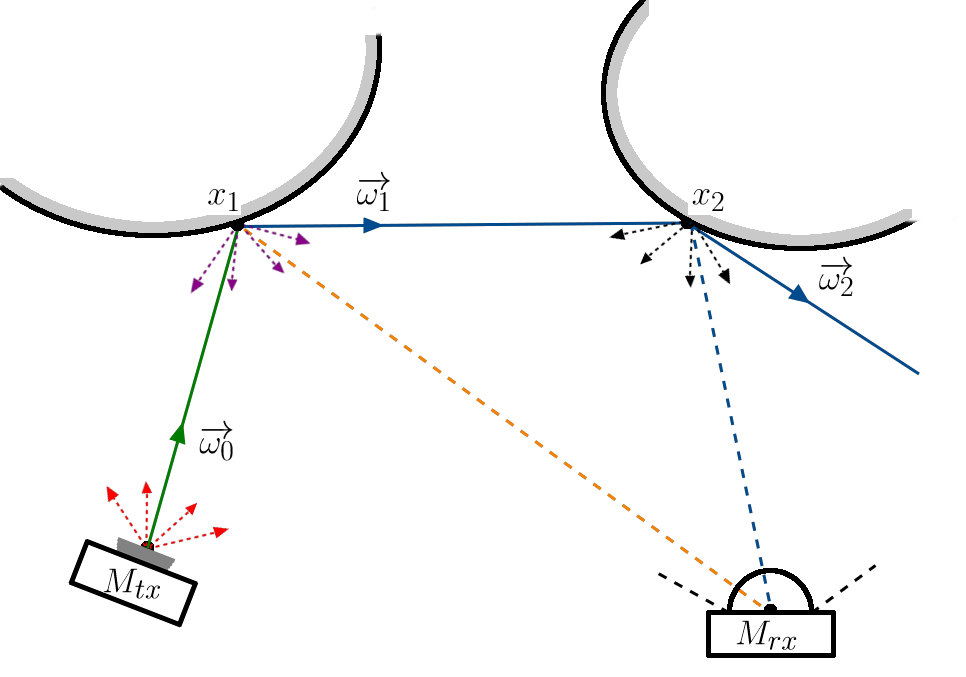
\includegraphics[width=150mm]{LTE.png}
\caption{Équation en potentiel avec la technique NEE}
\end{figure}


\large
\begin{equation}
    E(M_{tx}, M_{rx}, t) = \int_{\Omega_{tx}}
        \underbrace{\textcolor{OliveGreen}{L_e(M_{tx}, \overrightarrow{\omega_0}, t)}}
            _{\textcolor{DarkGray}
             {\substack{\text{rayonnement sortant} \\
                        \text{de $M_{tx}$ dans} \\
                        \text{la direction $\overrightarrow{\omega_0}$}}}}
        \underbrace{W(M_{tx}, M_{rx}, \overrightarrow{\omega_0}, t)}
            _{\textcolor{DarkGray}
             {\substack{\text{action potentielle de} \\
                        \text{la source $M_{tx}$ sur} \\
                        \text{le récepteur $M_{rx}$} \\
                        \text{dans la direction $\overrightarrow{\omega_0}$}}}}
        | \overrightarrow{\omega_0} \cdot \overrightarrow{n_{tx}} |
        \underbrace{\textcolor{red}{d\overrightarrow{\omega_0}}}
            _{\textcolor{DarkGray}
             {\substack{\text{intégrale} \\
                        \text{sur le} \\
                        \text{domaine} \\
                        \text{des} \\
                        \text{directions}}}}
.\end{equation} \normalsize

On tire un rayon de la source $M_{tx}$ dans la direction $\overrightarrow{\omega_0}$. Bien évidemment nous avons le rayonnement $L_e(M_{tx}, \overrightarrow{\omega_0}, t)$ sortant de la source, rayonnement atténué selon son inclinaison par rapport à la normale $\overrightarrow{n_{tx}}$ de la source. Ce rayonnement n'atteignant pas forcément le récepteur $M_{rx}$ immédiatement, il faut donc calculer l'action potentielle $W(M_{tx}, M_{rx}, \overrightarrow{\omega_0}, t)$ que la source a sur le récepteur par la direction $\overrightarrow{\omega_0}$.

\large \begin{multline}
    E(M_{tx}, M_{rx}, t) = \int_{\Omega_{tx}}
        \textcolor{OliveGreen}{L_e(M_{tx}, \overrightarrow{\omega_0}, t)}
        | \overrightarrow{\omega_0} \cdot \overrightarrow{n_{tx}} | \\
        \times \left(
        \underbrace{\textcolor{BurntOrange}{W_l^*(x_1, M_{rx}, t)}}
            _{\textcolor{DarkGray}
             {\substack{\text{contribution directe} \\
                        \text{de $x_1$ sur $M_{rx}$, en} \\
                        \text{tenant compte de la} \\
                        \text{BDRF}}}}
        + \int_{\Omega_1}
        \underbrace{\textcolor{blue}{W^*(x_1, M_{rx}, \overrightarrow{\omega_1}, t)}}
            _{\textcolor{DarkGray}
             {\substack{\text{contribution dans la direction} \\
                        \text{$\overrightarrow{\omega_1}$ en repartant de $x_1$} \\
                        \text{(à dérouler)}}}}
        \textcolor{purple}{d\overrightarrow{\omega_1}}
        \right)
        \textcolor{red}{d\overrightarrow{\omega_0}}
,\end{multline} \normalsize
avec
\large \begin{equation}
    W^*(x_1, M_{rx}, \overrightarrow{\omega_1}, t) = 
        f_r(x_1, \overrightarrow{\omega_0} \longrightarrow \overrightarrow{\omega_1})
        W(x_1, M_{rx}, \overrightarrow{\omega_1}, t)
        | \overrightarrow{\omega_1} \cdot \overrightarrow{n_1} |
,\end{equation} \normalsize
et
\large \begin{equation}
    W_l^*(x_1, M_{rx}, t) =
        f_r(x_1, \overrightarrow{\omega_0} \longrightarrow \overrightarrow{x_1 M_{rx}})
        W_l(x_1, M_{rx}, t)
        | \overrightarrow{\omega_1} \cdot \overrightarrow{n_1} |
.\end{equation} \normalsize

L'action potentielle $W(M_{tx}, M_{rx}, \overrightarrow{\omega_0}, t)$ se calcule en deux termes. Premièrement, sachant qu'en partant dans la direction $\overrightarrow{\omega_0}$ à partir du point $M_{tx}$ le rayon intercepte une surface au point de réflexion $x_1$, il faut regarder la contribution directe sur le récepteur de la lumière réfléchie en ce point; il s'agit du terme $W_l^*(x_1, M_{rx}, t)$. Ce premier terme ne traite donc que la direction de réflexion $\overrightarrow{x_1 M_{rx}}$.\par
Hors il y a tout un hémisphère de directions $\overrightarrow{\omega_1}$ possibles qu'il faut regarder. C'est ce que se charge de faire le deuxième terme $\int_{\Omega_1}W^*(x_1, M_{rx}, \overrightarrow{\omega_1}, t)d\overrightarrow{\omega_1}$. Ce terme là continue donc les chemins possibles du rayon et parmi toutes les directions, certaines iront intercepter d'autres surfaces (la direction $\omega_1$ qui intercepte une surface au point $x_2$ par exemple, sur la figure \ref{fig:LTE_potentiel}). C'est donc sur celui-ci qu'il faudra dérouler l'équation pour avoir $E_k(M_{tx}, M_{rx}, t)$.

\large \begin{multline} \label{eq:Eclairement_LTE_potentiel}
    E(M_{tx}, M_{rx}, t) =
        \int_{\Omega_{tx}}
            \textcolor{OliveGreen}{L_e(M_{tx}, \overrightarrow{\omega_0}, t)}
            \textcolor{BurntOrange}{W_l^*(x_1, M_{rx}, t)}
            | \overrightarrow{\omega_0} \cdot \overrightarrow{n_{tx}} |
            \textcolor{red}{d\overrightarrow{\omega_0}}
        \\ +
        \int_{\Omega_{tx}}
            \textcolor{OliveGreen}{L_e(M_{tx}, \overrightarrow{\omega_0}, t)}
            | \overrightarrow{\omega_0} \cdot \overrightarrow{n_{tx}} |
            \int_{\Omega_1}
                \textcolor{blue}{W^*(x_1, M_{rx}, \overrightarrow{\omega_1}, t)}
            \textcolor{red}{d\overrightarrow{\omega_0}}
        \textcolor{purple}{d\overrightarrow{\omega_1}}
.\end{multline} \normalsize

En séparant l'intégrale sur $\Omega_{tx}$ en deux intégrales, avec une seule à dérouler, nous pouvons facilement écrire l'équation pour $k$ réflexions.

\large \begin{equation}
\begin{split}
    E_k(M_{tx}, M_{rx}, t) =
        &\int_{\Omega_{tx}}
            f_1({M_{tx}, x_1, M_{rx}}, t)
        d\overrightarrow{\omega_0}
        \\ &+
        \int_{\Omega_{tx}}
            \int_{\Omega_1}
                f_2({M_{tx}, x_1, x_2,  M_{rx}}, t)
            d\overrightarrow{\omega_0}
        d\overrightarrow{\omega_1}
        \\ &\vdots
        \\ &+
        \int_{\Omega_{tx}}
            \cdots
            \int_{\Omega_k}
                f_k(\bar{x}, t)
            d\overrightarrow{\omega_0}
            \cdots
        d\overrightarrow{\omega_k}
.\end{split}
\end{equation} \normalsize \newline\par

Avec les intégrales sur les domaines de chemin, il est facile de voir que cette équation est très facilement transformable avec la méthode de Monte Carlo pour des facilités algorithmiques :
\large \begin{multline}
    E_k(M_{tx}, M_{rx}, t) =
    \frac{1}{N}
    \underbrace{
        \sum\limits_{s=1}^N \frac
            {| \overrightarrow{\omega_0} \cdot \overrightarrow{n_{tx}} |
             L_e(M_{tx}, \overrightarrow{\omega_{tx}}, t)}
            {p_0(M_{tx}, \overrightarrow{\omega_0})}
        }
        _{\textcolor{DarkGray}
         {\substack{\text{On tire une première} \\
                    \text{direction pour $\overrightarrow{\omega_0}$}}}}
    \\ \times
    \sum \limits_{i=1}^k
    \left(
        \underbrace
            {W_l(x_i, M_{rx}, t)}
            _{\textcolor{DarkGray}
             {\substack{\text{Contribution} \\
                        \text{directe du} \\
                        \text{point $x_i$ sur} \\
                        \text{le récepteur}}}}
        \underbrace
            {\prod\limits_{j=1}^i
                \frac
                    {f_r(x_j, \overrightarrow{\omega_{j-1}} \longrightarrow \overrightarrow{\omega_{j}})
                    | \overrightarrow{\omega_j} \cdot \overrightarrow{n_j} |}
                    {p_j(x_j, \overrightarrow{\omega_{j}})}}
                _{\textcolor{DarkGray}
                 {\substack{\text{Prise en compte de toutes} \\
                            \text{les BRDF des surfaces interceptées} \\
                            \text{par le chemin aux points $x_i$}}}}
    \right)
.\end{multline} \normalsize \newline\par
Cependant cette équation ne prend pour l'instant pas du tout en compte les milieux participants. Il s'agira donc ensuite de réfléchir à une solution pour injecter la distribution de la lumière par la fumée.

\section{Equation de rendu avec réflexions}

Rappelons l'équation de rendu (equation \ref{eq:LTE_rendu}) :
\large \begin{equation*}
    L_r(x, \overrightarrow{\omega_r}, t) =
        L_e(x, \overrightarrow{\omega_r}, t) +
        \int_{\Omega_x}
            f_r(x, \overrightarrow{\omega_i} \longrightarrow \overrightarrow{\omega_r})
            L_i(x, \overrightarrow{\omega_i}, t)
            |\overrightarrow{\omega_i}, \overrightarrow{n} |
        d\overrightarrow{\omega_i}
,\end{equation*} \normalsize
où $L_e(x, \overrightarrow{\omega_r}, t)$ est la lumière auto-émise par la surface, \\
$L_i(x, \overrightarrow{\omega_i}, t)$ est la radiance incidente dans la direction $\overrightarrow{\omega_i}$, \\
$\overrightarrow{n}$ est la normale à la surface au point $x$, \\
$f_r(x, \overrightarrow{\omega_i} \longrightarrow \overrightarrow{\omega_r})$ est la BRDF de la surface au point x dans le sens de propagation $\overrightarrow{\omega_i} \longrightarrow \overrightarrow{\omega_r}$.\newline\par

\begin{figure}[h!]\label{fig:LTE_rendu}
\centering
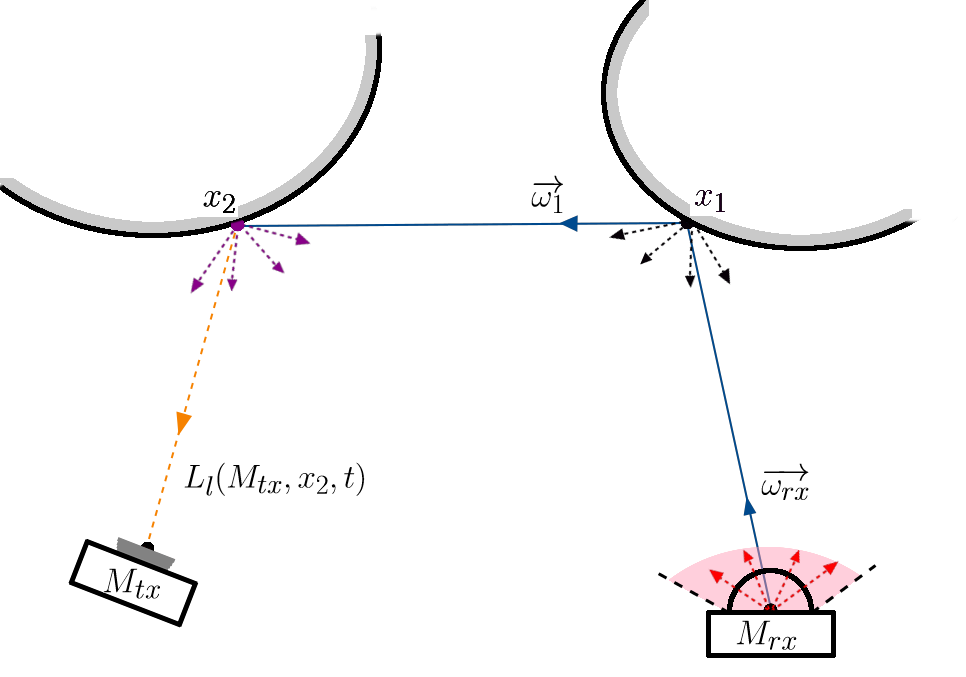
\includegraphics[width=150mm]{LTE_rendu.png}
\caption{Algorithme de rendu pour $k=2$ réflexions}
\end{figure}

Similairement à l'équation en potentiel, on va pouvoir en déduire l'éclairement reçu en un point $x$ après $k$ réflexions.\par
Après $k$ réflexions, on connecte le point de surface $x_k$ au récepteur. Ceci est représenté par la luminance rayonnée depuis l'émetteur $M_{tx}$ et reçue au dernier point de réflexion $x_k$ :
\large \begin{equation}
    L_l(M_{tx}, x_k, t) =
        L_e(M_{tx}, \overrightarrow{M_{tx}x_k}, t)
        V(x_k, M_{tx})
        \frac
            { | \overrightarrow{M_{tx}x_k}\cdot\overrightarrow{n_{tx}} | }
            { \| \overrightarrow{M_{tx}x_k} \| ^3}
.\end{equation} \normalsize \par
On rappelle que $V(x_k, M_{tx})$ est la fonction de visibilité qui vaut 1 si les points $x_k$ et $M_{tx}$ sont visibles l'un l'autre, 0 sinon.\newline\par

Nous voulons connaître l'éclairement reçu au récepteur, par le point de réflexion $x$. L'équation de rendu nous permet de modéliser la luminance réfléchie au point $x_1$ dans la direction $\overrightarrow{x_1 M_{rx}}$. En déroulant cette équation, nous arrivons pour $k$ réflexions à l'équation suivante :
\large \begin{equation}
    E_k(x_1, M_{rx}, t) =
        \int_{\textcolor{red}{\Omega_0}}
            \cdots
            \int_{\textcolor{purple}{\Omega_k}}
                g_k(\textcolor{blue}{\bar{x}}, t)
            \textcolor{red}{d\overrightarrow{\omega_0}}
            \cdots
        \textcolor{purple}{d\overrightarrow{\omega_k}}
,\end{equation} \normalsize
où $\bar{x} = (M_{rx}, x_1, x_2, ... , x_k, M_{tx})$ est un trajet partant du récepteur $M_{rx}$ et passant par $k$ points de réflexions avant d'atteindre la source $M_{tx}$. Et la fonction $g_k$ est:
\large \begin{multline}
    g_k(\bar{x}, t) =
        | \overrightarrow{\omega_0} \cdot \overrightarrow{n_{rx}} |
        rect\left(\frac
            {| \overrightarrow{\omega_0} \cdot \overrightarrow{n_{rx}} |}
            {cos(\textcolor{Rhodamine}{FOV})}
        \right) \\
        \times
        \textcolor{BurntOrange}{L_l(M_{tx}, x_k, t)}
        \prod\limits_{i=1}^k
            f_r(x_i, \overrightarrow{\omega_{i-1}} \longrightarrow \overrightarrow{\omega_{i}})
            | \overrightarrow{\omega_i} \cdot \overrightarrow{n_i} |
,\end{multline} \normalsize
où la fonction $rect$ vérifie que la direction $\overrightarrow{\omega_0}$ au champ de vision du récepteur, \\
le produit des BRDF $f_r(x_i, \overrightarrow{\omega_{i-1}} \longrightarrow \overrightarrow{\omega_{i}})$ à chaque point $x_i$ du trajet est un coefficient multiplicateur du dernier rayonnement en $x_k$.


\section{Equation de rendu optimisée}

Dans cet algorithme trivial on doit doit itérer plusieurs fois sur le même chemin si l'on souhaite avoir les contributions de chaque point de réflexion $x_i$ ($1 \leq i \leq k$) recevant directement de la lumière l'émetteur. On va donc, tout comme pour l'équation en potentiel, relier chaque point de réflexion à l'émetteur. Pour chaque point de réflexion $x_i$, si celui-ci peut recevoir une lumière directe de la source, la contribution de celle-ci est ajoutée avant de tirer une nouvelle direction aléatoire pour aller trouver un autre point de réflexion $x_{i+1}$.\newline\par

L'estimateur de Monte Carlo de cette version améliorée est le suivant :
\large \begin{multline}\label{eq:MC_LTE_rendu}
    E_k(M_{tx}, M_{rx}, t) =
    \frac{1}{N}
    \underbrace{
        \sum\limits_{s=1}^N \frac
            {| \overrightarrow{\omega_{rx}} \cdot \overrightarrow{n_{rx}} |}
            {p_0(M_{rx}, \overrightarrow{\omega_{rx}})}
        }
        _{\textcolor{DarkGray}
         {\substack{\text{On tire une première} \\
                    \text{direction pour $\overrightarrow{\omega_{rx}}$}}}}
    \\ \times
    \sum \limits_{i=1}^k
    \left(
        \underbrace
            {L_l(M_{tx}, x_i, t)}
            _{\textcolor{DarkGray}
             {\substack{\text{Contribution de} \\
                        \text{la source sur le} \\
                        \text{point $x_i$}}}}
        \underbrace
            {\prod\limits_{j=1}^i
                \frac
                    {f_r(x_j, \overrightarrow{\omega_{j-1}} \longrightarrow \overrightarrow{\omega_{j}})
                    | \overrightarrow{\omega_j} \cdot \overrightarrow{n_j} |}
                    {p_j(x_j, \overrightarrow{\omega_{j}})}}
                _{\textcolor{DarkGray}
                 {\substack{\text{Prise en compte de toutes} \\
                            \text{les BRDF des surfaces interceptées} \\
                            \text{par le chemin aux points $x_i$}}}}
    \right)
.\end{multline} \normalsize
\chapter{Fonctions de phase}

\section{Présentation}

Une BSDF (Bidirectional Scattering Distribution Function) permet de décrire et simuler la façon dont la lumière est dispersée par une surface. Une \textbf{fonction de phase} $\rho (\omega_{i}\longrightarrow\omega_{o})$ est son analogue volumétrique. Elle permet de décrire la façon dont la lumière se disperse \textit{à l'intérieur} du volume. On peut la lire comme une pdf donnant la probabilité qu'un photon arrivant sur une particule dans la direction $\omega_{i}$ en ressorte par la direction $\omega_{o}$. De ce fait, une fonction de phase possède une contrainte de normalisation :
\large \begin{equation}\label{eq:condition_de_normalisation}
    \int_{\Omega4\pi}\rho(\omega_{i}\longrightarrow\omega_{o})d\omega' = 1
.\end{equation} \normalsize \newline\par

Dans beaucoup de milieux participants, la fonction de phase est \textbf{isotropique}. Celle-ci ne dépend que de l'\textit{angle de phase} $\theta$ entre le rayon incident $\omega_{i}$ et le rayon sortant $\omega_{o}$. On se contente alors d'écrire $\rho(cos\theta)$. La dispersion est identique dans toutes les directions pour un angle donné.\par
Il est également intéressant de noter que les fonctions de phases sont des fonctions réciproques, les deux directions incidentes et sortantes peuvent être interchangées et la valeur de la fonction de phase restera la même :
\large \begin{equation}\label{eq:fp_reciprocité}
    \rho(\omega_{i}\longrightarrow\omega_{o}) = \rho(\omega_{o}\longrightarrow\omega_{i})
.\end{equation} \normalsize \newline\par


Tout comme les BSDF, il existe de nombreux modèles de fonctions de phase qui produisent des effets différents. Certains peuvent facilement être décrits avec un seul paramètre, mais d'autres plus complexes demandent une équation bien plus grosse et difficilement utilisables dans un algorithme. Il est donc parfois plus simple de diviser une fonction de phase $\rho(\omega_{i}\longrightarrow\omega_{o})$ complexe en plusieurs fonctions de phases $\rho_{k}(\omega_{i}\longrightarrow\omega_{o})$ plus simples. Nous avons l'égalité suivante :
\large \begin{equation}\label{eq:fp_somme}
    \rho(\omega_{i}\longrightarrow\omega_{o}) = \sum\limits_{k=1}^n w_{k}\rho_{k}(\omega_{i}\longrightarrow\omega_{o})
,\end{equation} \normalsize
où chacune des fonctions $\rho_{k}$ possède un poids $w_{k}$ dans l'équation, avec la somme de tous les $w_{k}$ qui égale 1 afin de maintenir la \textit{condition de normalisation} (formule \ref{eq:condition_de_normalisation}).


\section{Henyey-Greenstein}
\label{explication_parametre_g}

Henyey et Greenstein (1941) ont introduit une fonction de phase qui est aujourd'hui beaucoup utilisée car elle ne dépend que d'un paramètre $-1 \leq g \leq 1$ et décrit les effets de \textit{backscattering} tout comme ceux de \textit{forwardscattering} :
\large
$$\rho_{HG}(cos\theta) = \frac{1}{4\pi} \frac{1-g^2}{(1+g^2-2g(cos\theta))^{3/2}}.$$
\normalsize
Le paramètre $g$ n'est pas arbitraire et peut être calculé avec la formule suivante :
\large
$$g = \int_{\Omega4\pi}\rho(\omega_{i}\longrightarrow\omega_{o})(\omega_{i}\cdot\omega_{o})d\omega_{o} = 2\pi\int_{0}^{\pi}\rho(cos\theta)cos\theta sin\theta d\theta.$$
\normalsize
\par
La valeur de $g$ induit certains effets de dispersion dans la fonction de phase $\rho_{HG}$. Si $g<0$ alors la fonction de phase décrit principalement des effets de \textit{backscattering} (Figure \ref{fig:backscattering}). Si $g>0$, on a à l'inverse principalement du \textit{forwardscattering} (Figure \ref{fig:forwardscattering}). Enfin, comme on s'y attend, si $g=0$, la fonction de phase est isotropique.\newline\par

\begin{figure}
   \begin{minipage}[c]{.46\linewidth}
      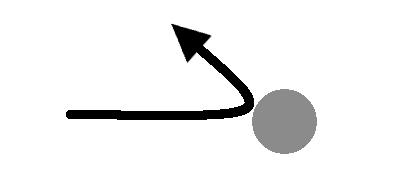
\includegraphics[width=80mm]{backscattering.png}
      \caption{Backscattering, $g<0$}
      \label{fig:backscattering}
   \end{minipage} \hfill
   \begin{minipage}[c]{.46\linewidth}
      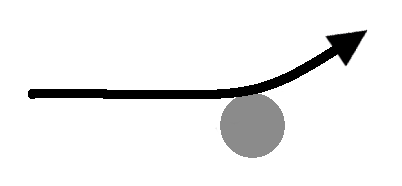
\includegraphics[width=80mm]{forwardscattering.png}
      \caption{Forwardscattering, $g>0$}
      \label{fig:forwardscattering}
   \end{minipage}
\end{figure}

\section{Schlick}

La fonction de phase de Henyey et Greenstein est cependant lourde à calculer à cause de la puissance présente au dénominateur. Blasi, Le Saëc et Schlick (1993) ont développé une approximation de $\rho_{HG}$ qui évite cette puissance et qui est donc plus utilisée en informatique graphique, où la forme exacte de la fonction de phase de Henyey et Greenstein n'est pas nécessaire.
\large
$$\rho_{Schlick}(cos\theta) = \frac{1}{4\pi} \frac{1-k^2}{(1-kcos\theta)^2},$$
\normalsize
où le paramètre $k$ joue le même rôle que le terme $g$ : $k=-1$  un backscattering total, $k=0$ implique l'isotropie du milieu, $k=1$ correspond à un forwardscattering total. Pharr et Humphreys (2004) ont trouvé que définir $k$ comme :
\large
$$k = 1,55g-0,55g^2,$$
\normalsize
était une bonne façon d'avoir une relation directe entre $k$ et $g$ avec laquelle $\rho_{Schlick}$ avoisine très bien $\rho_{HG}$.

\section{Rayleigh}

Le modèle de Rayleigh décrit une dispersion de la lumière dans un milieu composé de petites particules, jusqu'à un dixième de la longueur d'onde de la lumière.
\large
$$\rho_{R}(cos\theta) = \frac{3}{16\pi}(1+cos^2\theta).$$
\normalsize
Ce modèle permet par exemple de simuler la diffusion de la lumière dans le ciel. En le suivant, on retrouve ainsi sa couleur bleue.


\section{Mie}

La théorie de Rayleigh ne fonctionne que pour des particules de petites tailles. Lorsque celles-ci dépassent le dixième de leur longueur d'onde (aérosols, poussière, goutellettes d'eau), il faudrait passer à la théorie de Mie. Cela dit, son application est compliquée. La figure \ref{fig:cloud_pf} présente une fonction de phase pour un nuage, trouvée avec la théorie de Mie.

\begin{figure}[h!]
\centering
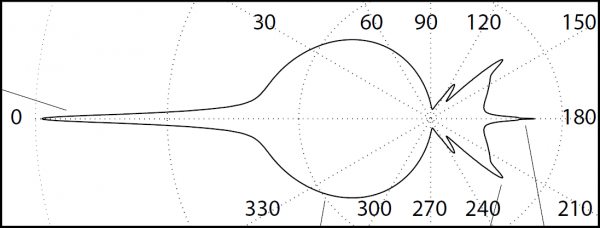
\includegraphics[width=150mm]{cloud_phase_function.png}
\caption{Fonction de phase d'un nuage}
\label{fig:cloud_pf}
\end{figure}

Aussi, plutôt que d'utiliser cette fonction de phase compliquée, on choisit généralement une composition de plusieurs fonctions de phase de Henyey et Greenstein (ou Schlick). C'est ici, par exemple, qu'est utilisée la formule \ref{eq:fp_somme} :
\large
$$\rho(\omega_{i}\longrightarrow\omega_{o}) = \sum\limits_{k=1}^n w_{k}\rho_{k}(\omega_{i}\longrightarrow\omega_{o}).$$
\normalsize
\chapter{Interactions}

Lorsque la lumière traverse un milieu participant, de multiples interactions peuvent avoir lieu au fur et à mesure que le rayon de lumière avance dans le milieu et rencontre des particules. La fréquence et la puissance de ces interactions vont dépendre de plusieurs propriétés du milieu participant, comme la densité par exemple. Ces propriétés varient dans le milieu, celui-ci étant rarement globalement homogène. Lorsque nous en seront à l'algorithme, il sera donc possible de décomposer le milieu en une grille 3D de fragments homogènes où les propriétés du milieu seront constantes.

\section{Absorption}

Lorsque la lumière arrive sur une particule, celle-ci fait obstruction et un certains nombres de photons ne parviennent donc pas à continuer leur chemin, c'est l'\textbf{absorption} (Figure \ref{fig:absorption}).

\begin{figure}[h!]\label{fig:absorption}
\centering
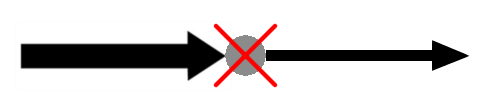
\includegraphics[width=100mm]{particule_absorption.png}
\caption{Absorption par une particule}
\end{figure}

Un milieu participant homogène possède un \textit{coefficient d'absorption} $\sigma_{a}$ qui correspond à la probabilité que la lumière soit absorbée lors de son passage dans le milieu. Une estimation simple et constante de ce coefficient est la suivante :
\large
$$\sigma_{a}(p, \omega) = \pi r^{2} N,$$
\normalsize
où $r$ est le rayon des particules (m) et $N$ la densité des particules (m$^{-3}$). $\sigma_{a}$ est donc en m$^{-1}$.

La valeur qui nous intéresse est la variation de radiance entre le faisceau arrivant sur la particule et celui en partant. Cette différence ne dépend que de la radiance initiale et du coefficient d'absorption du milieu traversé :
\large
\begin{equation}
    \Delta L(p, \omega) = L_{o}(p, \omega) - L_{i}(p, \omega) = -\sigma_{a}(p, \omega)L_{i}(p, \omega)dt
.\end{equation}
\normalsize

\section{Out-Scattering}

Lorsque le faisceau de lumière rencontre une particule dans le milieu, les photons qui le composent peuvent être absorbés (cf. Absorption) mais également renvoyés dans d'autres directions. C'est ce qu'on appelle l'\textbf{out-scattering} (figure \ref{fig:out_scattering}).

\begin{figure}[h!]\label{fig:out_scattering}
\centering
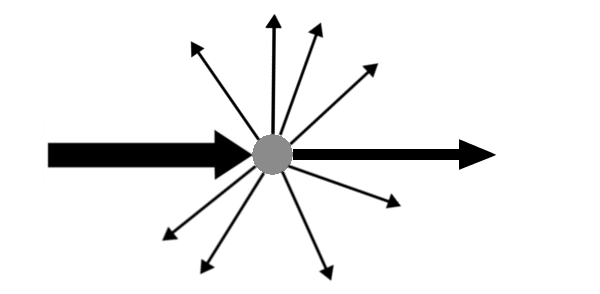
\includegraphics[width=100mm]{particule_out_scattering.png}
\caption{Out-scattering causé par une particule}
\end{figure}

Tout comme il existe un coefficient d'absorption, le milieu possède un \textit{coefficient de dispersion} $\sigma_{s}$ correspondant à la probabilité que le faisceau de lumière soit dispersé.

Son impact est semblable au coefficient d'absorption :
\large \begin{equation}
    \Delta L(p, \omega) = -\sigma_{s}(p, \omega)L_{i}(p, \omega)dt
.\end{equation} \normalsize

\section{Extinction}

Nous avons deux interactions qui atténuent la lumière lorsque celle-ci passe dans un milieu participant : l'absorption et l'out-scattering. Ces deux effets combinés donnent l'\textbf{extinction}. Un milieu participant homogène possède donc, de manière analogue aux deux interactions vues précédemment, un \textit{coefficient d'atténuation}, ou \textit{coefficient d'extinction} $\sigma_{t}$. Celui-ci est tout simplement donné par :
\large
$$\sigma_{t} = \sigma_{a} + \sigma_{s}.$$
\normalsize
Ce qui conduit à :
\large \begin{equation}
    \Delta L(p, \omega) = -\sigma_{t}(p, \omega)L_{i}(p, \omega)dt
.\end{equation} \normalsize \newline\par

Nous pouvons maintenant calculer non pas un delta de radiance mais une \textbf{proportion}. Soient $p$ et $p'$ deux points sur un rayon de direction normalisée $\omega$, à une distante $d$ l'un de l'autre. Alors nous avons :
\large \begin{equation} \label{eq:transmittance_definition}
    T_{r}(p\longrightarrow p') = e^{-\int_{0}^{d} \sigma_{t}(p+t\omega, \omega)dt} = e^{-\tau}
.\end{equation} \normalsize
où $T_{r}$ est la \textit{transmittance}, la proportion de radiance qui est transmise de $p$ à $p'$ sur un rayon traversant le milieu participant. $\tau$ est appelé l'\textit{épaisseur optique} du milieu. Sachant que dans un milieu homogène $\sigma_{t}$ est constant, on a $T_{r}(p\longrightarrow p') = e^{-\sigma_{t}d}$ : c'est la \textit{loi de Beer}.\par
Ainsi, soit $L_{o}(p, \omega)$ la radiance sortant d'un point $p$ d'une surface dans une direction normalisée $\omega$. Ce rayon traverse une milieu participant et arrive sur un autre point $p'$. Alors la radiance incidente à ce point $p'$ est donnée par (cf. figure \ref{fig:transmittance}) :
\large \begin{equation}
    L_{i}(p', -\omega) = T_{r}(p\longrightarrow p')L_{o}(p, \omega)
.\end{equation} \normalsize \par

Il va donc de soit que dans le vide, $T_{r}(p\longrightarrow p') = 1$.

\begin{figure}[h!]\label{fig:transmittance}
\centering
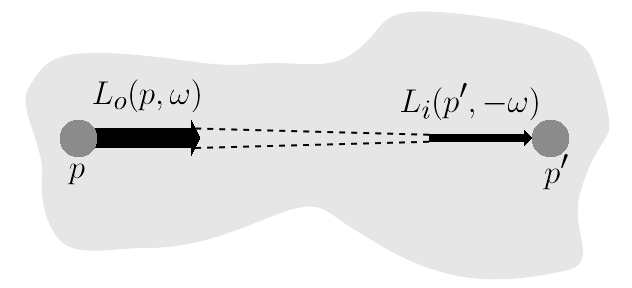
\includegraphics[width=100mm]{transmittance.png}
\caption{Atténuation d'un rayon grâce à la transmittance}
\end{figure}

Une propriété importante de la transmittance, qui nous sera utile pour l'écriture de l'algorithme, dit que la transmittance est multiplicative le long des points sur un rayon. Soient $p$ et $p''$ deux points sur un rayon. Et soit $p'$ un point entre $p$ et $p''$. Alors on a :
\large \begin{equation}
    T_{r}(p\longrightarrow p'') = T_{r}(p\longrightarrow p')T_{r}(p'\longrightarrow p'')
.\end{equation} \normalsize

\section{Émission}

Lors de son passage dans un milieu participant, la radiance du rayon ne fait pas que diminuer. Certains milieux participants peuvent auto émettre de la lumière. C'est ce qu'on appelle l'\textbf{émission} (figure \ref{fig:emission}). Lorsque le faisceau de lumière passe sur une particule émettant de la lumière, celui-ci gagne en intensité.

\begin{figure}[h!]\label{fig:emission}
\centering
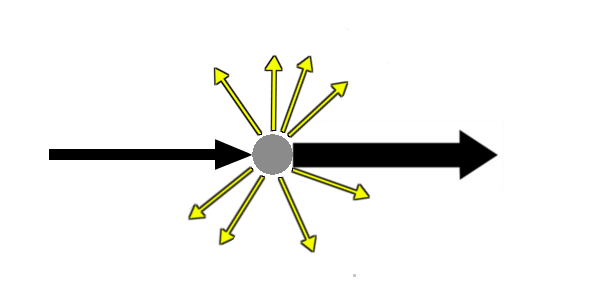
\includegraphics[width=100mm]{particule_emission.png}
\caption{Émission d'une particule}
\end{figure}

La lumière émise, qui ne dépend ici pas du rayon incident au point $p$ s'ajoute à la radiance :
\large \begin{equation}
    \Delta L(p, \omega) = L_{ve}(p, \omega)
.\end{equation} \normalsize

\section{In-Scattering}

Nous avons vu que lors d'une dispersion de la lumière (out-scattering), des photons étaient déviés de leur trajectoire, ne contribuant donc plus à la radiance du rayon initialement lancé. Ces photons ne disparaissent cependant pas et vont contribuer ailleurs, ils vont s'ajouter à un autre rayon avec qui ils partagent la trajectoire. Cela dit, il serait lourd de calculer, à chaque point p et chaque évènement d'out-scattering, les contributions de chaque nouveau rayon de contributions individuellement faibles. Pour simuler cet effet, nous avons donc l'interaction \textbf{in-scattering}(figure \ref{fig:in_scattering}).\par
Lorsque le faisceau rencontre une particule et que nous voulons calculer les contributions de chacune des interactions présentées précédemment, nous ajoutons la contribution des ces radiances perdues.

\begin{figure}[h!]\label{fig:in_scattering}
\centering
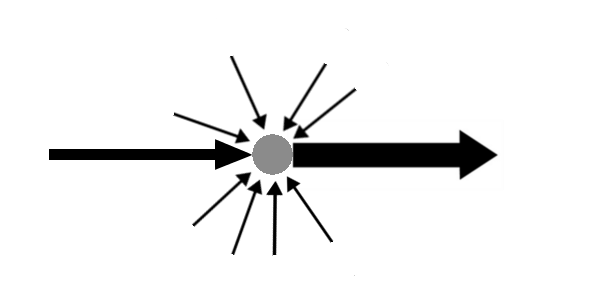
\includegraphics[width=100mm]{particule_in_scattering.png}
\caption{In-scattering sur une particule}
\end{figure}

Cet ajout dépend naturellement du \textit{coefficient de dispersion} $\sigma_{s}$, puisque l'\textit{out-scattering} et l'\textit{in-scattering} sont dûs à la même réaction.\par

Le calcul de cett interaction est cependant un peu plus complexe. En effet, là où pour l'out-scattering nous n'avions pas besoin de savoir ce qu'il se passait de la radiance perdue, nous devons ici prendre en compte que nouveaux rayons qui ont voyagé dans le milieu avant d'arriver jusqu'à notre particule, et dont ma direction a changé. C'est ici que nous utilisons la \textbf{fonction de phase} $\rho$ de notre milieu :
\large \begin{equation}
  \Delta L(p, \omega) = \sigma_{s}(p, \omega) \int_{\Omega4\pi}\rho(p, -\omega'\longrightarrow\omega)d\omega' dt  
.\end{equation} \normalsize \par

Le domaine d'intégration est ici la sphère complète autour du point $p$. Puisque nous ne sommes pas sur une surface, il n'y a en effet pas d'obstruction faite ne laissant qu'une hémisphère de possibilités.

\section{Source}

Au final, nous avons deux interactions qui viennent augmenter la radiance d'un rayon lors de son passage dans un milieu participant : l'émission et l'in-scattering. Cela nous donne la \textbf{source} $L_s$ de radiance qui va venir s'ajouter à la radiance initiale :
\large \begin{equation}\label{eq:source}
    L_s(p, \omega) = L_{ve}(p, \omega) + \sigma_{s}(p, \omega) \int_{\Omega4\pi}\rho(p, -\omega'\longrightarrow\omega)L_i(p, \omega')d\omega'
.\end{equation} \normalsize
En découle :
\large \begin{equation}
    \Delta L(p, \omega) = L_s(p, \omega)dt
.\end{equation} \normalsize
\chapter{Équation de transfert}

Avec toutes ces interactions causées par le passage de la lumière dans un milieu participant, nous pouvons écrire l'\textbf{équation de transfert}. Cette équation va nous permettre de décrire le comportement et la distribution de la lumière dans le milieu. L'équation du transport de la lumière (LTE) est assez proche de ce que nous allons écrire, puisqu'il s'agit en fait d'une équation de transfert mais sans milieu participant.\newline\par

La différence entre la radiance incidente à un point $p$ selon la direction $\omega$  et la radiance sortante de ce point $p$ est tout simplement calculable grâce à l'extinction et la source causées par le milieu :
\large \begin{equation}
    \Delta L(p, \omega) = [-\sigma_{t}(p, \omega)L_{i}(p, \omega) + L_s(p, \omega)]dt
.\end{equation} \normalsize
\par

Rappelons que nous avons donc dans cette équation l'ensemble des quatre interactions :
\large \begin{multline}
    \frac{\Delta L(p, \omega)}{dt} =
        \underbrace{-
            \underbrace{\sigma_{a}(p, \omega)L_{i}(p, \omega)}_{absorption}-
            \underbrace{\sigma_{s}(p, \omega)L_{i}(p, \omega)}_{out-scattering}}
        _{extinction}
        \\ +
        \underbrace{
            \underbrace{L_{ve}(p, \omega)}_{emission}+
            \underbrace{\sigma_{s}(p, \omega) \int_{\Omega4\pi}\rho(p, -\omega'\longrightarrow\omega)L_i(p, \omega')d\omega'}_{in-scattering}}
        _{source}
.\end{multline}
\normalsize\newline\par

De là, il y a plusieurs moyens d'utiliser cette équation. Supposons qu'aucune surface ne vienne bloquer le rayon et que celui-ci soit donc de longueur infinie. Alors la radiance incidente à un point $p$ dans une direction $\omega$ est augmentée par la radiance $S$ ajoutée à chaque point $p'$ le long du rayon. Cette quantité de radiance ajoutée est réduite par la transmittance $T_{r}$. Nous aurons donc :
\large \begin{equation*}
L_{i}(p, \omega) = \int_{0}^{\infty} T_{r}(p'\longrightarrow p)L_s(p', -\omega) dt.
\end{equation*} \normalsize \newline\par

Supposons maintenant qu'il y ait présence de surfaces. Alors d'une part ces surfaces vont interagir avec les radiances du milieu par réflection et/ou émission et donc ajouter une contribution dans l'équation finale. Et d'autre part, elles peuvent empêcher complètement un rayon de continuer son chemin et donc enlever la contribution directe de ce rayon de l'autre côté de la surface.\par
Soit un rayon d'origine $p$ et de direction $\omega$ qui intercepte une surface au point $p_{0}$ (on a $p_{0} = p + t\omega$ où $t$ est la distance entre les deux points). Alors l'équation de transfert est la suivante :
\large \begin{equation} \label{eq:equation_of_transfert}
L_{i}(p, \omega) = T_{r}(p_{0}\longrightarrow p)L_{o}(p_{0}, -\omega) + \int_{0}^{t} T_{r}(p'\longrightarrow p)L_s(p', -\omega) dt'.
\end{equation} \normalsize
où $p' = p + t'\omega$ sont les points le long du rayon entre $p$ et $p_{0}$\par
Le premier terme de cette équation,  $T_{r}(p_{0}\longrightarrow p)L_{o}(p_{0}, -\omega)$,  correspond à la radiance réfléchie par la surface en $p_{0}$ dans la direction $-\omega$. C'est dans ce terme que la contribution de la surface est ajoutée (réflexion et émission sont compris dans $L_{o}$). Le second terme est celui bien connu maintenant, causé par les différentes interactions ayant eu lieu lors du passage de la lumière dans le média.
\chapter{Modification du code}

\section{Package participatingmedia}

J'ai ajouté un package \textbf{\textit{org.xlim.sic.ig.simulators.impl.participatingmedia}} dans lequel j'ai ajouté tous les fichiers que j'ai créés. S'y trouve donc l'arborescence suivante :\newline\newline
\begin{forest}
  for tree={
    font=\ttfamily,
    grow'=0,
    child anchor=west,
    parent anchor=south,
    anchor=west,
    calign=first,
    edge path={
      \noexpand\path [draw, \forestoption{edge}]
      (!u.south west) +(7.5pt,0) |- node[fill,inner sep=1.25pt] {} (.child anchor)\forestoption{edge label};
    },
    before typesetting nodes={
      if n=1
        {insert before={[,phantom]}}
        {}
    },
    fit=band,
    before computing xy={l=15pt},
  }
[participatingmedia
    [mcshooting1
        [RayShootingPPSimulator1.java]
        [RayShootingPPSimulatorFactory1.java]
    ]
    [mcshooting2
        [RayShootingPPSimulator2.java]
        [RayShootingPPSimulatorFactory2.java]
    ]
    [mcshooting3
        [RayShootingPPSimulator3.java]
        [RayShootingPPSimulatorFactory3.java]
    ]
    [ParticipatingMedia.java]
]
\end{forest}\newline\par
Chaque sous-package \textbf{\textit{mcshootingX}} correspond à un algorithme présenté ci-dessous. Durant la durée de mon stage, j'ai eu le temps de travailler sur les 3 premiers seulement.\newline\par

La classe \textbf{ParticipatingMedia} est commune à tous les algorithmes et sert à décrire un milieu participant. C'est ici que se trouvent les différentes méthodes pour calculer la transmittance, l'in-scattering, l'out-scattering, ...



\section{Modifications d'interfaces}

Il m'aura fallut modifier quelques interfaces déjà existantes du code.\newline\par

\textit{org.xlim.sic.ig.kernel.physics.\textbf{Brdf}} \qquad
En effet, la classe BRDF permettait de réaliser la réflexion pour un champ (lumineux, radio, ...) mais pas pour une réponse impulsionnelle. Hors, dans mon algorithme 2, mon lancer de rayon transporte une réponse impulsionnelle et non plus seulement un champ lumineux. Il me faut donc ajouter la méthode \textbf{reflect} qui prend en paramètre une réponse impulsionnelle (et qui pour chaque champ va lui appliquer la méthode \textbf{reflect} de base). Pour l'instant, je n'ai modifié que les implémentations utilisant des LightField.\newline\par

\textit{org.xlim.sic.ig.sensors.\textbf{Receiver}} \qquad
Là encore, un receiver ne pouvait recevoir qu'un champ et pas une réponse impulsionnelle. J'ai donc ajouté la méthode \textbf{receive} qui prend en paramètre une réponse impulsionnelle. Pour l'instant, seul le DiscReceiver a cette méthode implémentée.\newline\par

\textit{org.xlim.sic.ig.simulators.\textbf{ImpulseResponse}} \qquad
J'ai ajouté ici trois méthodes nécessaires pour l'algo 2 : \textbf{multiplyByAScalar} qui multiplie tous les champs de la réponse par un scalaire, \textbf{incrementDepth} qui décale de +1 en profondeur tous les champs de la réponse, \textbf{addTime} qui déplace dans le temps tous les champs de la réponse.
\chapter{Algorithme 1}

\section{Présentation}

Cet algorithme reprend l'algorithme MCS (ou MCG) classique avec la technique NEE, si ce n'est qu'entre deux points de réflexions on prend en compte l'atténuation de la fumée. Cette prise en compte est également faite entre la source et les différents points de surface, ou entre le récepteur et les différents points de surface.

\section{Intégration continue}

Entre deux points $p$ et $p'$, dans la direction $\omega$ ($p' = p + t\omega$), le rayon passe dans de la fumée et de ce fait nous avons la formule suivante :
\large \begin{equation}
    L_i(p', \omega) = T_r(p \rightarrow p')L_o(p, \omega)
.\end{equation} \normalsize \par
Rappelons ici la défintion de la transmittance $T_r$ (eq. \ref{eq:transmittance_definition}) :
\large \begin{equation}
    T_{r}(p\longrightarrow p') = e^{-\int_{0}^{d} \sigma_{t}(p+t\omega, \omega)dt}
.\end{equation} \normalsize

Dans cet algorithme, c'est le seul calcul que nous ferons, pour chaque luminance sortant d'un point de réflexion (ou de la source) et arrivant sur un autre point de réflexion (ou sur l'émetteur).\par
Rappelons l'équation \ref{eq:Eclairement_LTE_potentiel} pour l'algorithme MCS avec NEE :
\large \begin{multline*}
    E(M_{tx}, M_{rx}, t) =
        \int_{\Omega_{tx}}
            L_e(M_{tx}, \overrightarrow{\omega_0}, t)
            W_l^*(x_1, M_{rx}, t)
            | \overrightarrow{\omega_0} \cdot \overrightarrow{n_{tx}} |
            d\overrightarrow{\omega_0}
        \\ +
        \int_{\Omega_{tx}}
            L_e(M_{tx}, \overrightarrow{\omega_0}, t)
            | \overrightarrow{\omega_0} \cdot \overrightarrow{n_{tx}} |
            \int_{\Omega_1}
                W^*(x_1, M_{rx}, \overrightarrow{\omega_1}, t)
            d\overrightarrow{\omega_0}
        d\overrightarrow{\omega_1}
,\end{multline*} \normalsize
avec
\large \begin{equation*}
    W_l^*(x_1, M_{rx}, t) =
        f_r(x_1, \overrightarrow{\omega_0} \longrightarrow \overrightarrow{x_1 M_{rx}})
        W_l(x_1, M_{rx}, t)
        | \overrightarrow{\omega_1} \cdot \overrightarrow{n_1} |
,\end{equation*} \normalsize
et
\large \begin{equation*}
    W^*(x_1, M_{rx}, \overrightarrow{\omega_1}, t) = 
        f_r(x_1, \overrightarrow{\omega_0} \longrightarrow \overrightarrow{\omega_1})
        W(x_1, M_{rx}, \overrightarrow{\omega_1}, t)
        | \overrightarrow{\omega_1} \cdot \overrightarrow{n_1} |
.\end{equation*} \normalsize \newline \par

En ajoutant la prise en compte de la fumée, nous aurons :
\large \begin{multline}
    E(M_{tx}, M_{rx}, t) =
        \int_{\Omega_{tx}}
            \textcolor{red}{T_r(M_{tx} \rightarrow x_1)}
            L_e(M_{tx}, \overrightarrow{\omega_0}, t)
            W_l^*(x_1, M_{rx}, t)
            | \overrightarrow{\omega_0} \cdot \overrightarrow{n_{tx}} |
            d\overrightarrow{\omega_0}
        \\ +
        \int_{\Omega_{tx}}
            \textcolor{red}{T_r(M_{rx} \rightarrow x_1)}
            L_e(M_{tx}, \overrightarrow{\omega_0}, t)
            | \overrightarrow{\omega_0} \cdot \overrightarrow{n_{tx}} |
            \int_{\Omega_1}
                W^*(x_1, M_{rx}, \overrightarrow{\omega_1}, t)
            d\overrightarrow{\omega_0}
        d\overrightarrow{\omega_1}
,\end{multline} \normalsize
avec
\large \begin{equation*}
    W_l^*(x_1, M_{rx}, t) =
        \textcolor{red}{T_r(x_1 \rightarrow M_{r_x})}
        f_r(x_1, \overrightarrow{\omega_0} \longrightarrow \overrightarrow{x_1 M_{rx}})
        W_l(x_1, M_{rx}, t)
        | \overrightarrow{\omega_1} \cdot \overrightarrow{n_1} |
,\end{equation*} \normalsize
et
\large \begin{equation*}
    W^*(x_1, M_{rx}, \overrightarrow{\omega_1}, t) = 
        f_r(x_1, \overrightarrow{\omega_0} \longrightarrow \overrightarrow{\omega_1})
        W(x_1, M_{rx}, \overrightarrow{\omega_1}, t)
        | \overrightarrow{\omega_1} \cdot \overrightarrow{n_1} |
,\end{equation*} \normalsize
où
\large \begin{equation*}
    W(x, y, \overrightarrow{\omega_x}, t) =
        \textcolor{red}{T_r(x \rightarrow y)}
        W_e(x, y, \overrightarrow{\omega_x}, t) +
        \int_{\Omega_z}
            f_r(z, \overrightarrow{\omega_x} \longrightarrow \overrightarrow{\omega_z})
            W(z, y, \overrightarrow{\omega_z}, t)
            |\overrightarrow{\omega_z}, \overrightarrow{n_z} |
        d\overrightarrow{\omega_z}
.\end{equation*} \normalsize

\section{Implémentation discrète}

Cette intégrale peut être transformée avec Monte Carlo :

\large \begin{multline}
    E_k(M_{tx}, M_{rx}, t) =
    \frac{1}{N}
    \underbrace{
        \sum\limits_{s=1}^N \frac
            {| \overrightarrow{\omega_0} \cdot \overrightarrow{n_{tx}} |
             \textcolor{red}{T_r(M_{tx} \rightarrow x_1)}
             L_e(M_{tx}, \overrightarrow{\omega_{tx}}, t)}
            {p_0(M_{tx}, \overrightarrow{\omega_0})}
        }
        _{\textcolor{DarkGray}
         {\substack{\text{On tire une première} \\
                    \text{direction pour $\overrightarrow{\omega_0}$}}}}
    \\ \times
    \sum \limits_{i=1}^k
    \left(
        \underbrace
            {W_l(x_i, M_{rx}, t)}
            _{\textcolor{DarkGray}
             {\substack{\text{Contribution} \\
                        \text{directe du} \\
                        \text{point $x_i$ sur} \\
                        \text{le récepteur}}}}
        \underbrace
            {\prod\limits_{j=1}^i
                \frac{
                    \textcolor{red}{T_r(x_j \rightarrow x_{j-1})}
                    f_r(x_j, \overrightarrow{\omega_{j-1}} \longrightarrow \overrightarrow{\omega_{j}})
                    | \overrightarrow{\omega_j} \cdot \overrightarrow{n_j} |}
                    {p_j(x_j, \overrightarrow{\omega_{j}})}}
                _{\textcolor{DarkGray}
                 {\substack{\text{Prise en compte de toutes les BRDF} \\
                            \text{des surfaces interceptées, et de la} \\
                            \text{fumée entre les différents sommets du chemin}}}}
    \right)
.\end{multline} \normalsize



\section{Algorithme}

Dans ma classe \textbf{ParticipatingMedia}, j'ai ajouté la méthode \textbf{\textit{multiplyByTransmittance}} qui, pour une distance $d$ donnée, multiplie des champs par la transmittance $tr = e^{-\sigma_t d}$ (possible car nous sommes dans un milieu homogène).\par
Ensuite, cette méthode est appliquée sur chaque rayon produit par l'algorithme de lancer de rayons.

\section{Résultats}

Dans cet algorithme, puisque le seul impact de la fumée est l'extinction par la transmittance, nous n'avons pas à différencier les coefficients d'atténuation $\sigma_a$ et de dispersion $\sigma_s$. En effet, le seul qui nous intéresse est $\sigma_t = \sigma_a + \sigma_s$.\par
Les résultats qui suivent ont été réalisés avec $10^8$ rayons lancés, 3 réflexions, et 4 valeurs différentes de $\sigma_t$. Ils sont présentés dans un premier temps, par réflexion (seulement le trajet direct, seulement la première réflexion, ...) puis toutes les contributions sont rassemblées.

\begin{center}
\begin{figure}[h!]
      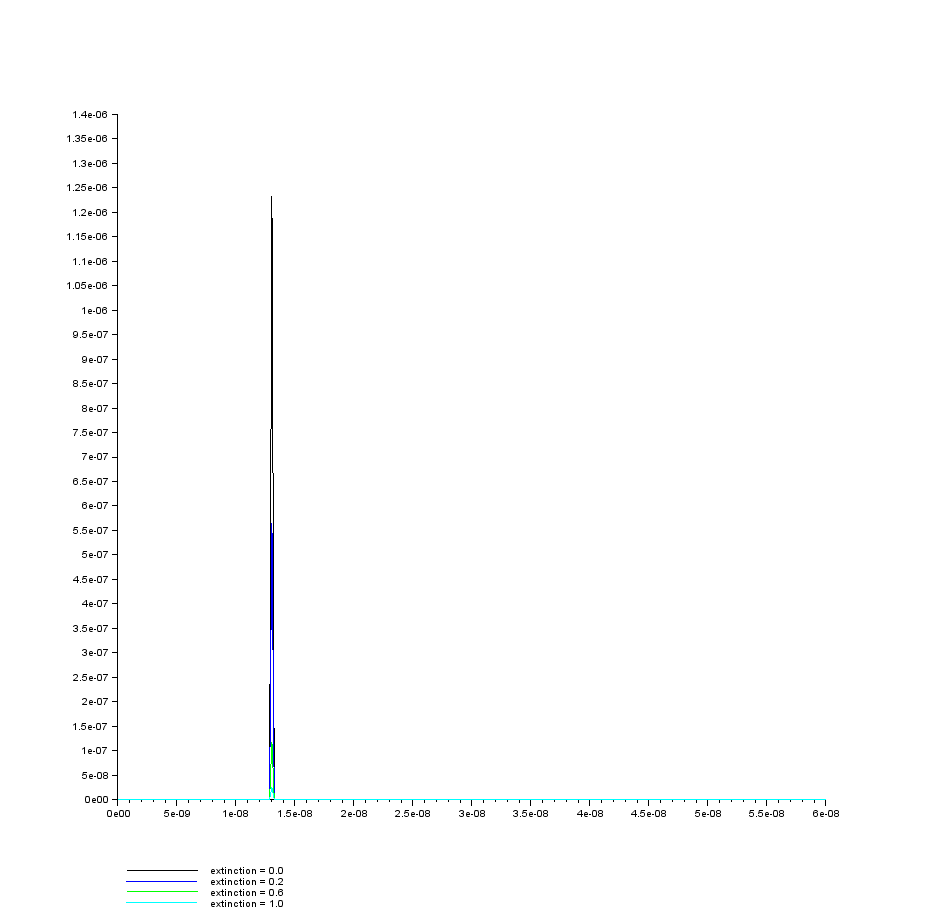
\includegraphics[width = 180mm]{resultats/algo1/depth0.png}
      \caption{k = 0}
\end{figure}
\begin{figure}[h!]
      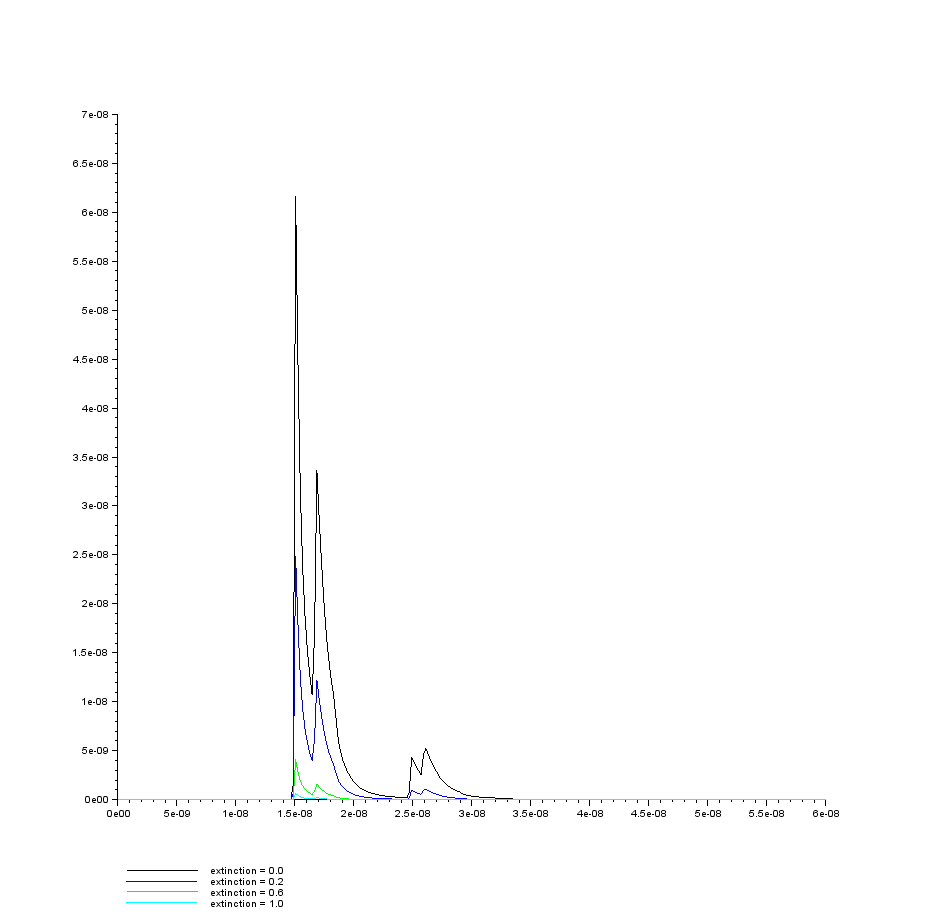
\includegraphics[width = 19cm]{resultats/algo1/depth1.png}
      \caption{k = 1}
\end{figure}
\begin{figure}[h!]
      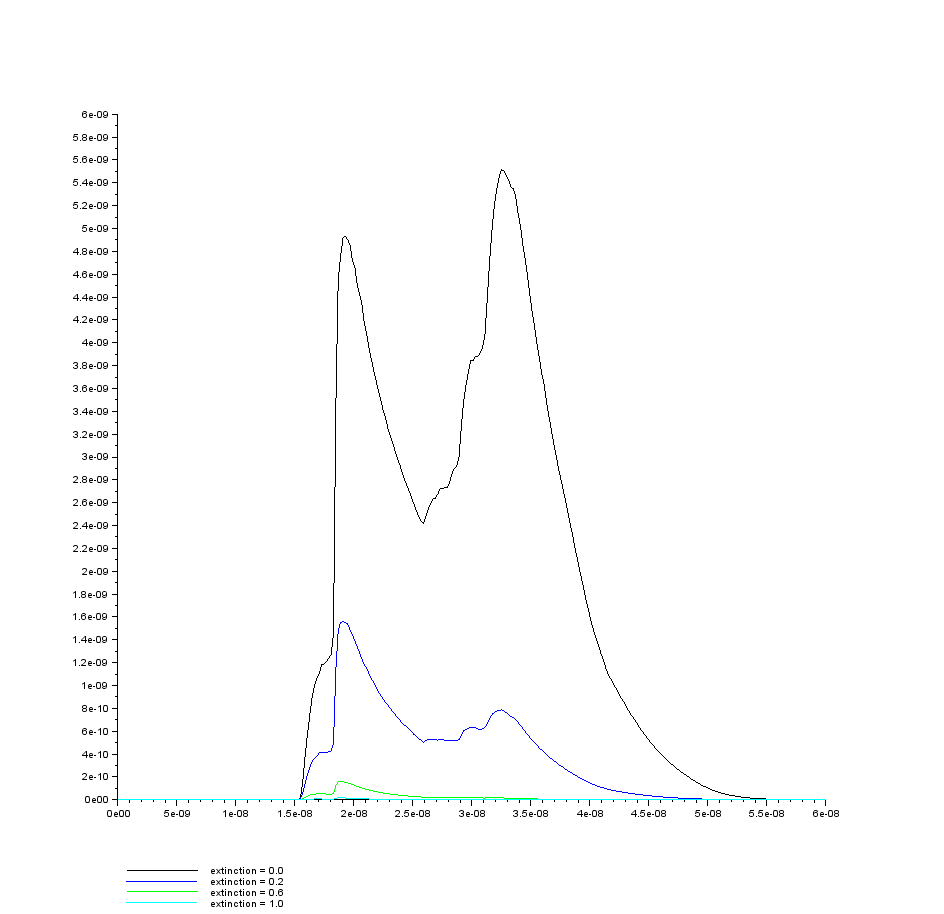
\includegraphics[width = 19cm]{resultats/algo1/depth2.png}
      \caption{k = 2}
\end{figure}
\begin{figure}[h!]
      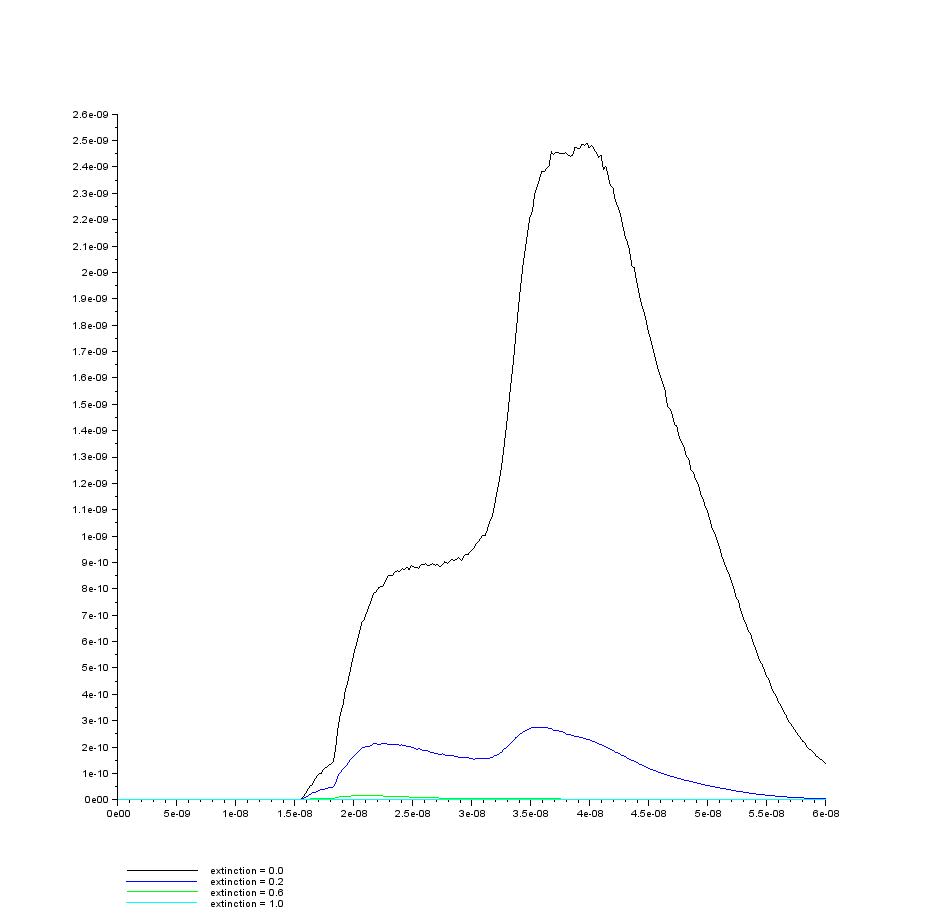
\includegraphics[width = 19cm]{resultats/algo1/depth3.png}
      \caption{k = 3}
\end{figure}
\begin{figure}[h!]
      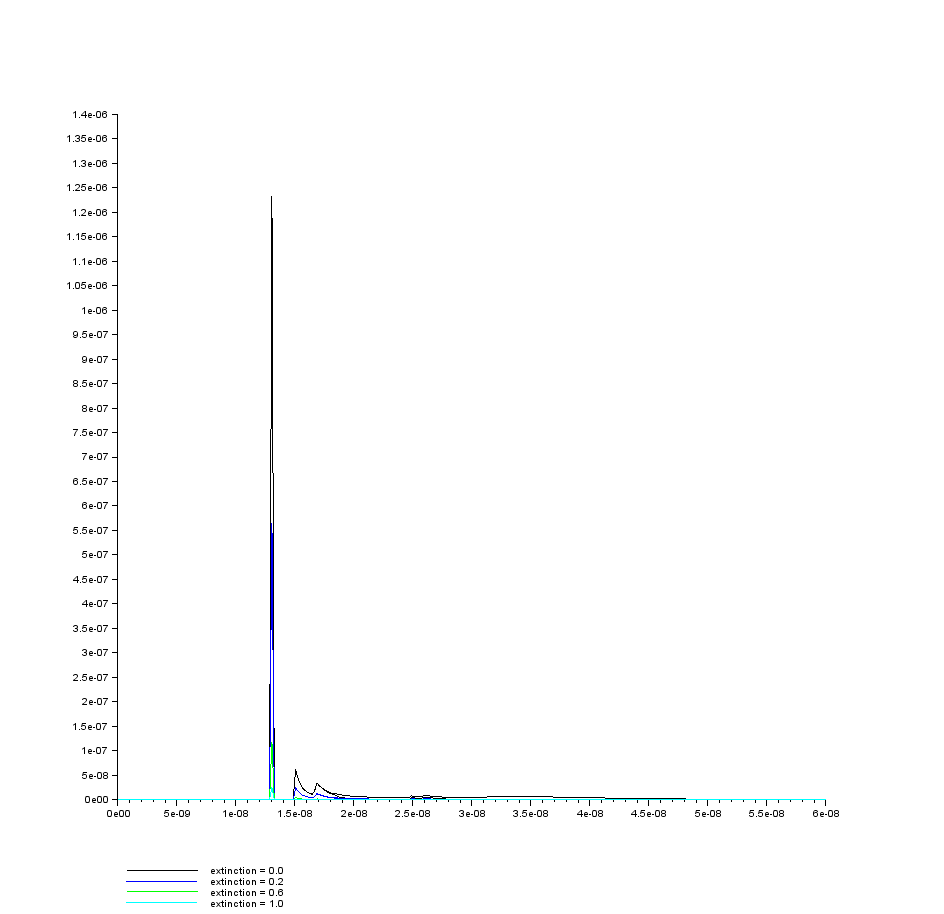
\includegraphics[width = 19cm]{resultats/algo1/alldepth.png}
      \caption{k = 0, 1, 2, 3}
\end{figure}
\end{center}
\chapter{Algorithme 2}

\section{Présentation}

Le deuxième algorithme reprend le premier algorithme mais décompose chaque rayon entre deux points de surface (ou émetteur/récepteur) en plusieurs segments afin de prendre en compte l'in-scattering provenant de la source (et uniquement de la source) à plusieurs endroits dans la fumée.

\section{Intégration continue}

Prenons un rayon qui après un rebond sur une surface au point $x_i$, repart dans une direction $\omega_i$ pour arriver au point $x_{i+1}$. Alors la luminance arrivant sur le point $x_{i+1}$ et portée par ce rayon est donnée par (eq. \ref{eq:equation_of_transfert}) :
\large \begin{equation*}
    L_i(x_{i+1}, \omega_i) =
        T_r(x_i \longrightarrow x_{i+1})
        L_o(x_i, \omega_i)
        +
        \int_0^t
            T_r(x_i\longrightarrow p')
            L_s(p', \omega_i)
        dt'
.\end{equation*} \normalsize \newline\par

Dans notre cas, nous n'avons pas de lumière émise par la fumée. Seul l'in-scattering intervient et le terme $L_s$ devient donc :
\large \begin{equation*}
    L_s(p, \omega) =
        \sigma_s(p, \omega)
        \int_{\mathcal{S}^2}
            \rho(p, \omega' \longrightarrow \omega)
            L_i(p, \omega')
        d\omega'
.\end{equation*} \normalsize \par

De plus, les $L_i$ venant des différentes directions $\omega_i$ ne sont pas connues dans un premier temps. La seule direction incidente pour laquelle il est possible d'avoir une valeur (autre que la direction $\omega$) est la direction $\overrightarrow{M_{tx}p_k}$ de la source au point $p_k$. Nous n'avons plus qu'un seul choix de direction incidente, il n'est plus nécessaire d'avoir du Monte Carlo et la source devient donc :
\large \begin{equation} \label{eq:source_algo_1}
    L_s(p, \omega) =
        \sigma_{s}(p, \omega)
        \rho(p, \overrightarrow{M_{tx}p} \longrightarrow \omega)
        L_d(p)
,\end{equation} \normalsize
où $L_d(p)$ est la luminance venant directement de la source :
\large \begin{equation}
    L_d(p) = T_r(M_{tx} \longrightarrow p) L_e(M_{tx}, \omega)
.\end{equation} \normalsize

\section{Découpe du rayon}

Le lumière traversant la fumée va rencontrer de nombreuses particules avant d'arriver sur une surface. Il serait lourd de réaliser autant de calculs qu'il n'y a de particules sur le chemin du rayon, mais d'un autre côté ne réaliser qu'un seul calcul serait très inexact. Il faut donc découper ce rayon en plusieurs points $p_i$ séparés d'une distance à trouver de manière cohérente. Mon rayon, lancé au point $p$ et touchant une surface au point $p'$ est donc décomposé comme le montre la figure \ref{fig:decomposition_rayon}.

\begin{figure}[h!]
\centering
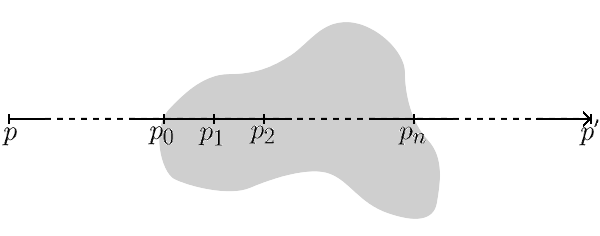
\includegraphics[width=150mm]{ray_decomposition.png}
\caption{Décomposition du rayon}
\label{fig:decomposition_rayon}
\end{figure}

Nous connaissons le point de départ $p$ et le point d'arrivée $p'$ du rayon. Nous pouvons donc connaître le temps $t$ qui correspond à l'arrivée de la lumière sur le récepteur, après avoir effectué le chemin $(M_{tx}, p, M_{r_x})$. Il en va de même pour le temps $t'$ pas le chemin $(M_{tx}, p, p', M_{r_x})$. Avec ces deux données temporelles, il est possible de déduire les positions des points intermédiaires $p_k$, et plus précisément leur distance à $p$, afin d'obtenir des potentiels répartis régulièrement entre $t$ et $t'$, selon une durée $\Delta t$ qui est un paramètre de la simulation. (cf. figure \ref{fig:find_ray_decomposition})

\begin{figure}[h!]
\centering
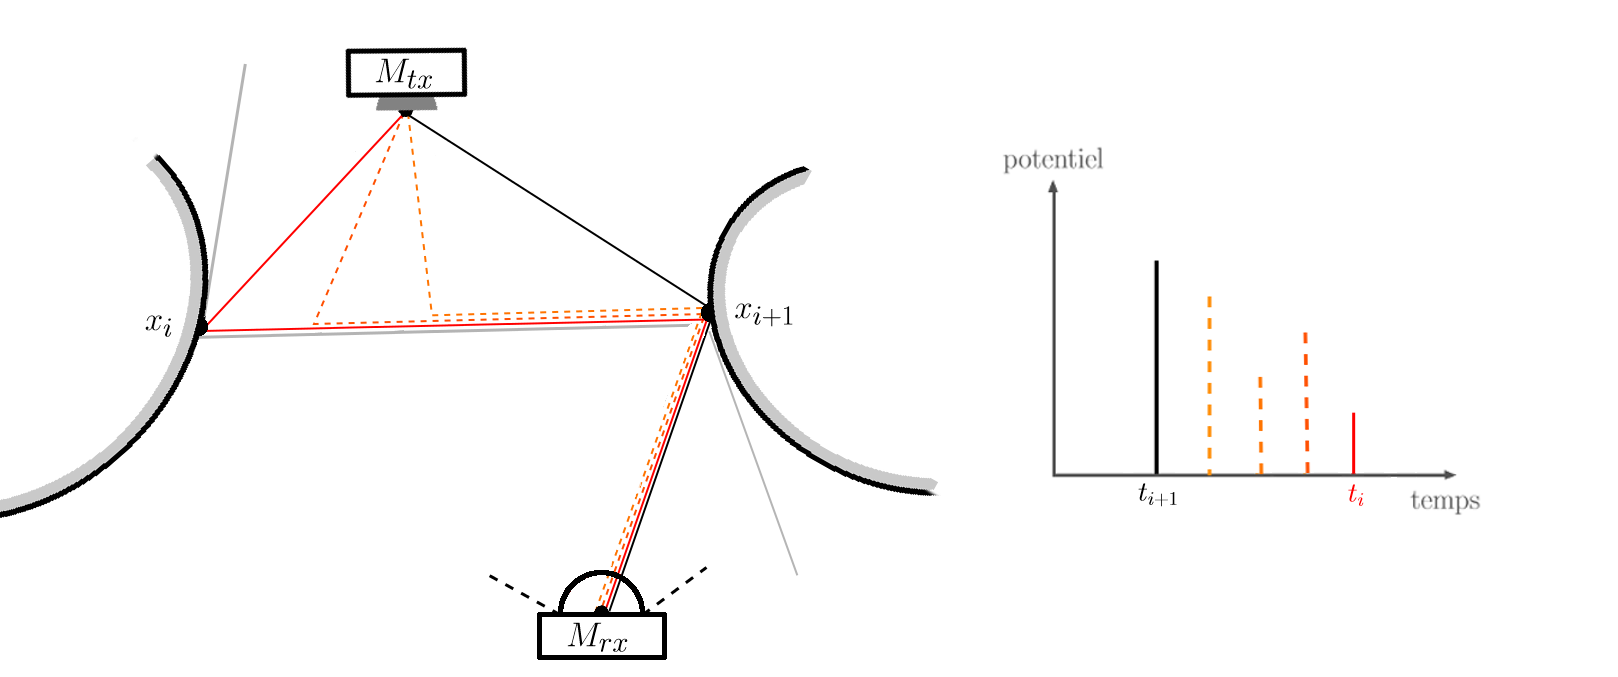
\includegraphics[width=180mm]{find_ray_decomposition_Tx.png}
\caption{Décomposition du rayon et réponse impulsive correspondante}
\label{fig:find_ray_decomposition}
\end{figure}

Pour réaliser la découpe de ce rayon, j'utilise les équations de l'ellipse. En effet, l'inconnue que nous cherchons c'est la distance entre $x_i$ et un point intermédiaire $p$ sur le rayon de direction $\overrightarrow{x_i x_{i+1}}$. Nous connaissons la distance entre $x_i$ et $M_{t_x}$, notons-la $d1$, qui sont des points fixes. Nous connaissons également la longueur totale $L = x_i p + p M_{tx}$, que l'on peut trouver en calculant les temps $t_i$ et $t_{i+1}$. Cette distance étant fixée, nous sommes dans un problème d'ellipse : deux foyers ($x_i$ et $M_{tx}$) et un paramètre (la longueur $L$). Connaissant l'angle $\theta = \angle M_{tx} x_i p$, l'inconnue $r(\theta) = x_i p$ est donc calculable car il s'agit de la distance entre un point de l'ellipse et un foyer, 

\begin{figure}[h!]
\centering
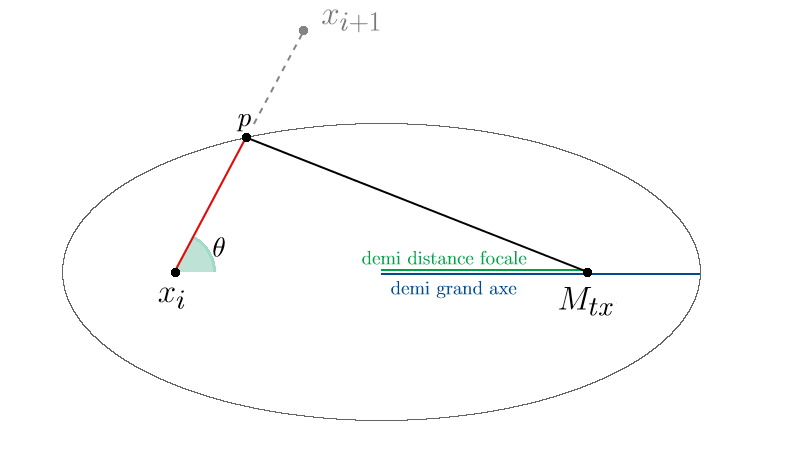
\includegraphics[width=180mm]{ellipseTx.png}
\caption{Utilisation de l'ellipse pour trouver la distance $x_i p$}
\end{figure}

Voici les équations utilisées pour cela :
\begin{itemize}
    \item La longueur du chemin passant par le point $p$ est notée $L = x_i p + p M_{tx}$
    \item La longueur du demi grand-axe est noté $a = L/2$
    \item La distance séparant le centre de l'ellipse et un des foyers, notée $c = x_i M_{tx} / 2$ est la demi-distance focale
    \item L'excentricité est $e = c/a$
    \item Le "paramètre" de l'ellipse est $\gamma = a(1-e^2)$
    \item Enfin, l'équation polaire d'une éclipse nous donne $r(\theta) = \frac{\gamma}{1 + e cos\theta}$
\end{itemize} \par

Ce qui amène l'algorithme suivant :
\begin{lstlisting}[language=java]
private double[] computeStepSizeIn(Ray ray, double stepTime){
    // distance de la source au debut du rayon (de M_tx a x_i)
    double d1 = Ray.createFromFromAndTo(this.irf.transmitter.getPosition(), ray.from).getDistance();
    // distance de la source a la fin du rayon (de M_tx a x_{i+1})
    double d2 = Ray.createFromFromAndTo(this.irf.transmitter.getPosition(), ray.to).getDistance();
    
    // Il va maintenant falloir trouver l'angle theta.
    // Pour cela, on va d'abord chercher la hauteur du triangle (x_i - p - M_tx)
    // en utilisant la formule de Heron
    double perimeter = d1 + d2 + ray.getDistance();
    double p = perimeter/2.0;
    double area = Math.sqrt(p * (p-d1) * (p-d2) * (p-ray.getDistance()));
    double h = area * 2.0 / ray.getDistance(); // la hauteur provenant de la source M_tx
    
    // On peut maintenant trouver l'angle theta avec la formule de trigonometrie suivante :
    // dans un triangle rectangle, nous avons
    // sin(angle) = (longueur du cote oppose)/(longueur de l'hypothenuse)
    // Ici, l'angle theta est celui du sommet x_i
    double theta = Math.asin(h/d1);
    
    // On peut egalement calculer les temsp t1 et t2
    double t1 = d2/physics.getSpeed();
    double t2 = (d1 + ray.getDistance())/physics.getSpeed();
    
    // et en deduire le nombre de points intermediaires qu'il doit y avoir
    // entre x_i et x_{i+1}
    int nbPoints = (int)Math.floor((t2 - t1)/stepTime);
    double[] distancesToRayStart = new double[nbPoints+1];
    
    double[] L = new double[nbPoints+1];
    distancesToRayStart[0] = 0D;
    // pour chaque point, on va pouvoir derouler les equations presentees plus haut
    for (int i = 1; i < distancesToRayStart.length - 1; ++i){
        L[i] = (t1 + i*stepTime) * physics.getSpeed();
    
        // Ellipse
        double a = L[i]/2D; // grand axe
        double c = d1/2D; // demi-distance focale
        double e = c/a; // excentricite
        // utilisation de l'equation polaire
        double A_X = (a*(1-e*e))/(1+e*Math.cos(theta));
        distancesToRayStart[i] = A_X;
    }
    distancesToRayStart[distancesToRayStart.length - 1] = ray.getDistance();
    return distancesToRayStart;
}
\end{lstlisting}

\section{Problème de temporalité}

Je choisis intentionnellement de commencer ma décomposition à l'entrée du milieu participant. En effet, entre $p$ et $p_{0}$, aucune particule ne viendra modifier la radiance et nous avons donc :
$$L_{o}(p, \omega) = L_{i}(p_{0}, \omega).$$\par
De la même manière, à la sortie du milieu participant il ne sert plus à rien de décomposer. Nous aurons :
$$L_{i}(p', \omega) = L_{o}(p_{n}, \omega).$$\par
Bien évidemment, il est tout à fait possible de fusionner $p$ et $p_0$ si dans un premier temps on considère que la fumée remplit toute la scène. Dans ce cas, $p'$ se trouvera aussi dans la fumée et on calculera $L_{i}(p', \omega)$ comme n'importe quel $L_{i}(p_i, \omega)$.

Avec ce que nous savons, nous pourrions décomposer le calcul de la radiance en $n+1$ itérations, en suivant ce schéma :
\large \begin{align*}
L_{i}(p_{0}, \omega) &= L_{o}(p, \omega) ,\\
L_{o}(p_{0}, \omega) &= L_{i}(p_{0}, \omega) - \sigma_{t}(p_{0}, \omega)L_{i}(p_{0}, \omega) + L_s(p_{0}, \omega) ,\\
L_{i}(p_{1}, \omega) &= T_{r}(p_{0}\longrightarrow p_{1})L_{o}(p_{0}, \omega) ,\\
L_{o}(p_{1}, \omega) &= L_{i}(p_{1}, \omega) - \sigma_{t}(p_{1}, \omega)L_{i}(p_{1}, \omega) + L_s(p_{1}, \omega) ,\\
... \\
L_{i}(p_{n}, \omega) &= T_{r}(p_{n-1}\longrightarrow p_{n})L_{o}(p_{n-1}, \omega) ,\\
L_{o}(p_{n}, \omega) &= L_{i}(p_{n}, \omega) - \sigma_{t}(p_{n}, \omega)L_{i}(p_{n}, \omega) + L_s(p_{n}, \omega) ,\\
L_{i}(p', \omega) &= L_{o}(p_{n}, \omega)
.\end{align*} \normalsize\newline\par

Plus généralement, mise à part éventuellement aux extrémités de la décomposition, nous aurions les deux calculs suivants sur lesquels il faudrait itérer (cf. figure \ref{fig:zoom_pk}) :
\large \begin{align}
    \label{eq:deroulement_Li}
    L_{i}(p_{k}, \omega) &= T_{r}(p_{k-1}\longrightarrow p_{k})L_{o}(p_{k-1}, \omega) ,\\
    \label{eq:deroulement_Lo}
    L_{o}(p_{k}, \omega) &= L_{i}(p_{k}, \omega)(1 - \sigma_{t}(p_{k}, \omega)) + L_s(p_{k}, \omega)
.\end{align} \normalsize

\begin{figure}[h!]
\centering
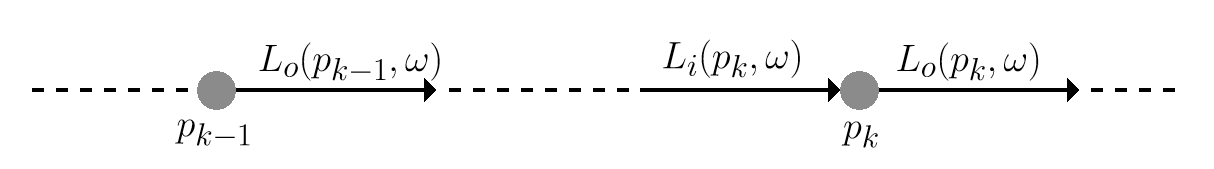
\includegraphics[width=150mm]{zoom_pk.png}
\caption{Zoom sur la décomposition}
\label{fig:zoom_pk}
\end{figure}

Mais il faut prendre en compte que la lumière provenant directement de la source et correspondant à notre in-scattering, ne parcours pas le même chemin que le rayon initialement lancé qui a effectué plusieurs réflexions (figure \ref{fig:different_paths}). Le récepteur ne recevra pas leurs contribution au même moment (figure \ref{fig:different_times}). Il n'est donc pas possible d'itérer comme présenté précédemment puisque $L_s(p_3, \omega)$ ne correspond pas au même pic de potentiel que $L_o(p_2, \omega)$ par exemple.\par
Il faudra compléter la réponse impulsionnelle pour chaque point intermédiaire $p_k$ à des temporalités différentes. Et non pas sommer toutes les contributions, dues à l'in-scattering, sur une même temporalité.

\begin{figure}[h!]
\centering
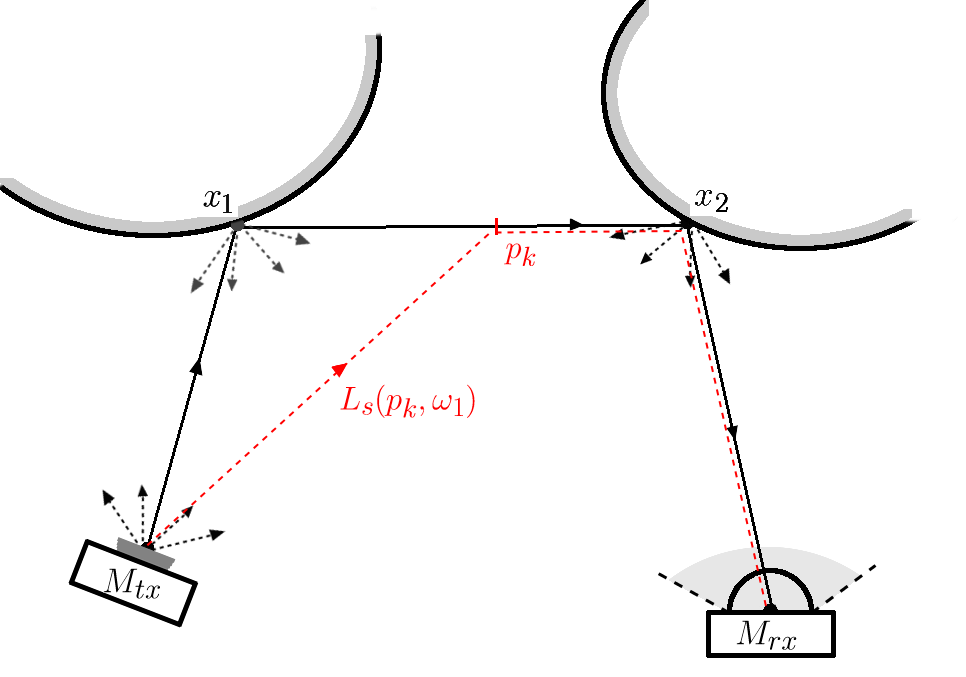
\includegraphics[width=150mm]{time_difference.png}
\caption{Le chemin des réflexions (ligne pleine) est plus long que celui débuté par l'in-scattering (pointillés)}
\label{fig:different_paths}
\end{figure}

\begin{figure}[h!]
\centering
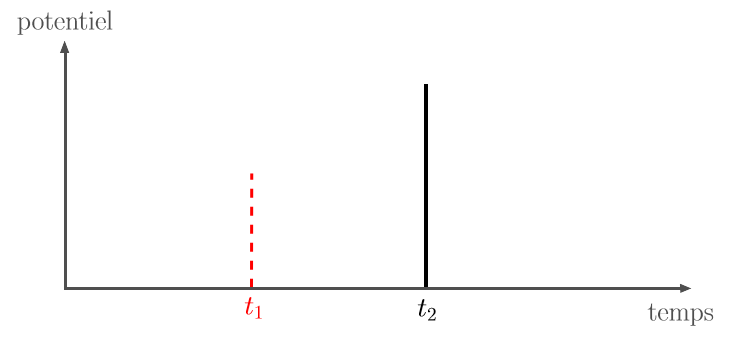
\includegraphics[width=130mm]{potentiel_graph.png}
\caption{La contribution de l'in-scattering est donc reçue plus tôt en $M_{rx}$}
\label{fig:different_times}
\end{figure}

\newpage

\section{Algorithme}

Dans ma classe \textit{\textbf{ParticipatingMedia}}, j'ajoute une méthode qui sera utilisée pour trouver la réponse impulsionnelle finale.

\paragraph{inScatteringAlongARay} Cette méthode calcule la contribution de la source en plusieurs points le long du rayon de direction $\omega$ : c'est l'in-scattering. Pour chaque point intermédiaire $p_i$ (appelons-les \textit{point de milieu} en opposition aux \textit{points de surface}, je calcule la source grâce à la fonction de phase appliquée au point $p_i$ sur le rayon $\omega$. Je multiplie cette source $L_s(p_i, \omega)$ par la transmittance car elle passe également dans la fumée avant d'atteindre le point $p_i$. Puis finalement, j'ajoute cette contribution lumineuse à la réponse impulsionnelle qui sera réutilisée dans une nouvelle itération de la méthode \textbf{RayLaunching}. \newline\par

J'utilise toujours la méthode suivante :

\paragraph{multiplyByTransmittance} Cette méthode ne s'occupe pas de l'in-scattering mais de l'extinction le long du rayon. Puisque ceci correspond au trajet de base du rayon (entre deux points de réflexions trouvé dans la méthode \textbf{RayLaunching}), il n'y a pas besoin de s'occuper de la réponse impulsionnelle ici. En effet, ceci est déjà géré dans la méthode \textbf{RayLaunching}. \newline\newline\par

Il aura également fallut que je modifie la classe \textit{\textbf{ImpulseResponse}} en y ajoutant deux méthodes.

\paragraph{addTime} Après avoir calculé une réponse impulsionnelle potentielle comprenant tout l'in-scattering entre deux points de réflexions $x_i$ et $x_{i-1}$, l'algorithme réalise un rebond vers un autre point de réflexion $x_{i+2}$. Ce nouveau rayon est une distance supplémentaire parcourue par les contributions d'in-scattering sur tous les rayons précédents. Il faut donc, dans la réponse impulsionnelle potentielle, décaler tous les champs en fonction de cette nouvelle longueur. Cette méthode prend donc en paramètre un temps. Il s'agit de la distance du nouveau rayon obtenu après rebond, divisé par la vitesse de la lumière. Et met à jour la réponse impulsionnelle.

\paragraph{addDepth} De la même manière, lorsque ce rebond est effectué, la distance du chemin augmente mais le nombre de réflexions également. L'in-scattering, lorsqu'il est calculé sur le rayon de direction $\omega_i$, est ajouté à une profondeur de 1 puisqu'il ne correspond à aucune réflexion (il vient directement de la source sur un point de milieu sur le rayon), et ceux peut importe le rayon $\omega_i$ sur lequel on travaille. A chaque rebond, il faut donc indiquer que ces contributions ajoutées préalablement dans la réponse impulsionnelle potentielle, effectuent un rebond de plus.


\section{Résultats}

Incorrects pour l'instant. Travail en cours.
\chapter{Algorithme 3}

\section{Présentation}

Le troisième algorithme applique la technique du NEE en chaque point intermédiaire. Ainsi, chaque point $p_k$ sera connecté au récepteur où sa contribution sera prise en compte.

\section{Découpe du rayon}

Ici, il faut procéder comme pur l'algorithme 3, mais les foyers de l'ellipse seront les point $x_i$ et $M_{rx}$ puisque nous voulons connecter chaque point intermédiaire $p$ au récepteur afin d'appliquer le NEE (et non plus à l'émetteur).

\begin{figure}[h!]
\centering
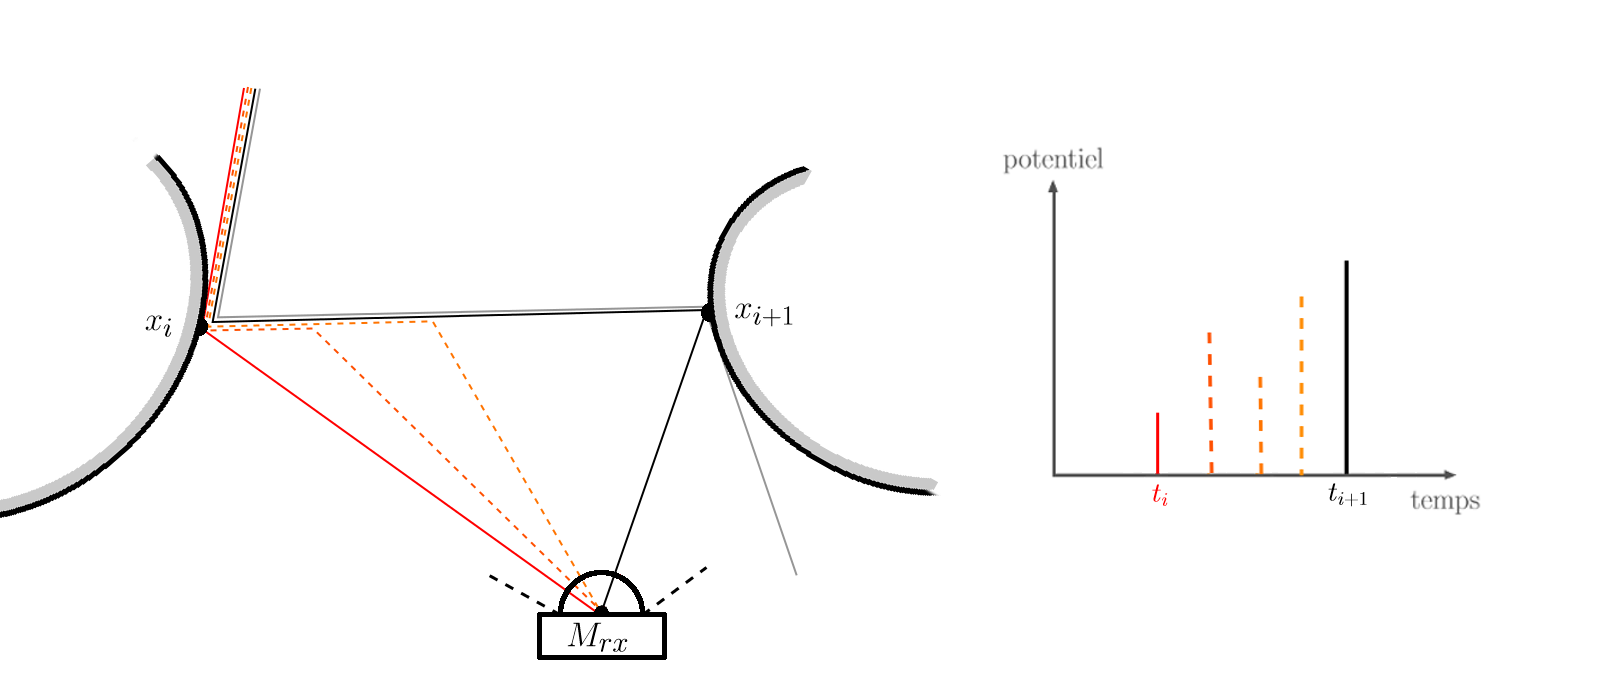
\includegraphics[width=180mm]{find_ray_decomposition_Rx.png}
\caption{Décomposition du rayon et réponse impulsive correspondante}
\end{figure}

\begin{figure}[h!]
\centering
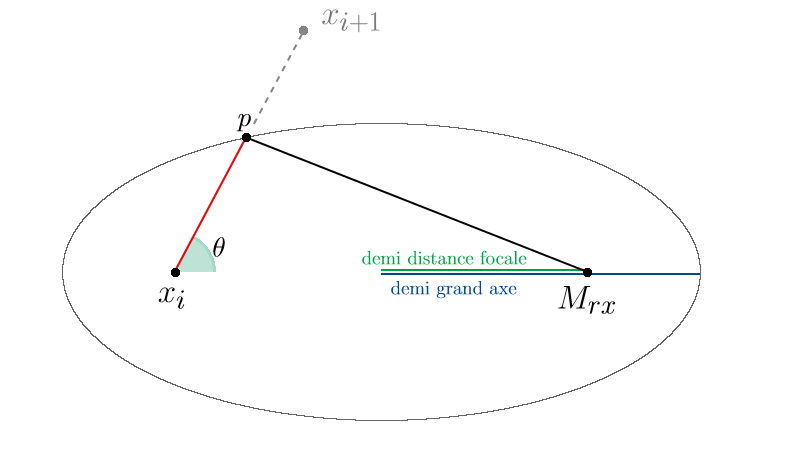
\includegraphics[width=180mm]{ellipseRx.png}
\caption{Utilisation de l'ellipse pour trouver la distance $x_i p$}
\end{figure}

\section{Algorithme}

Je rajoute, une méthode \textbf{outScatteringAlongARay} qui gère la connexion au récepteur $M_{rx}$ pour chaque point intermédiaire (point de milieu), en simulant la réception par le récepteur, et en complétant la réponse impulsionnelle.

\section{Résultats}

Suite à un problème avec Scilab, je n'ai pas pu réaliser des graphes comme à l'algo 1, c'est-à-dire un graphe par profondeur.

\subsection{Coefficient de dispersion}

Dans un premier temps, nous regardons l'impact du coefficient de dispersion sur les contributions lumineuses. Ainsi :
\begin{itemize}
    \item le coefficient d'atténuation $\sigma_a$ vaut 0 ;
    \item le paramètre g vaut 0 : le milieu est complètement isotropique.
    \item la densité du milieu est de 1 ;
    \item 3 réflexions.
\end{itemize}
\vspace{1em}\par

En lançant $10^7$ rayons, nous obtenons le résultat de la figure \ref{fig:resultats_algo3_dispersion}.\newline

\begin{figure}[h!]
\centering
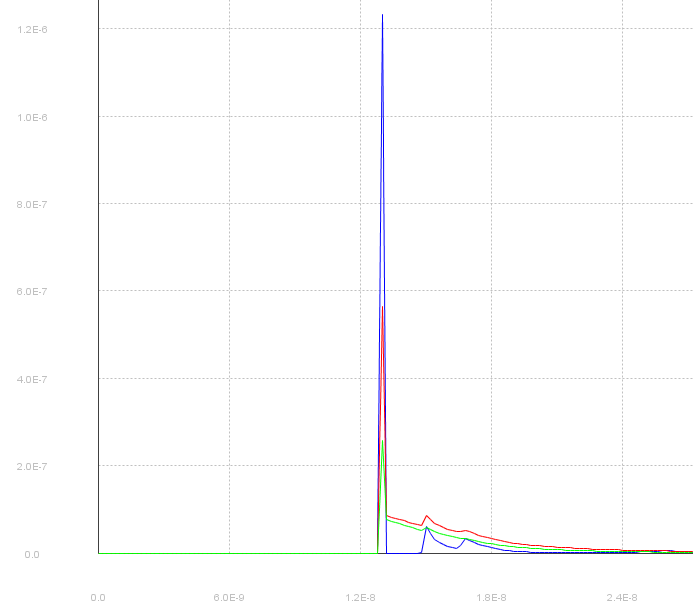
\includegraphics[width=150mm]{resultats/algo3/algo_3_resultats.PNG}
\caption{
bleu : $\sigma_s = 0.0$ \qquad
rouge : $\sigma_s = 0.2$ \qquad
vert : $\sigma_s = 0.4$}
\label{fig:resultats_algo3_dispersion}
\end{figure}

On remarque que l'out-scattering produit dans un premier temps un effet d'amplification de la lumière. Le récepteur reçoit en permanence des rayons qui viennent contribuer, même faiblement. Cela dit, au bout d'un moment le coefficient d'extinction devient trop fort et la lumière est tellement atténuée que les contributions de l'out-scattering ne sont plus suffisantes pour avoir un gain de lumière.

\subsection{Paramètre g}

Rappelons que le paramètre $g$ d'un milieu participant indique si celui-ci est isotropic ($g = 0$), induit une majorité de backward-scattering ($-1 < g < 0$) ou une majorité de forward-scattering ($0 < g < 1$) (cf section \ref{explication_parametre_g}).\par
Pour les résultats suivants, je n'ai fait varier que le paramètre g et les autres valeurs étaient :
\begin{itemize}
    \item le coefficient d'atténuation $\sigma_a$ vaut 0 ;
    \item le coefficient de dispersion $\sigma_s$ vaut 0.2 ;
    \item la densité du milieu est de 1 ;
    \item 3 réflexions.
\end{itemize}

\begin{figure}[h!]
\centering
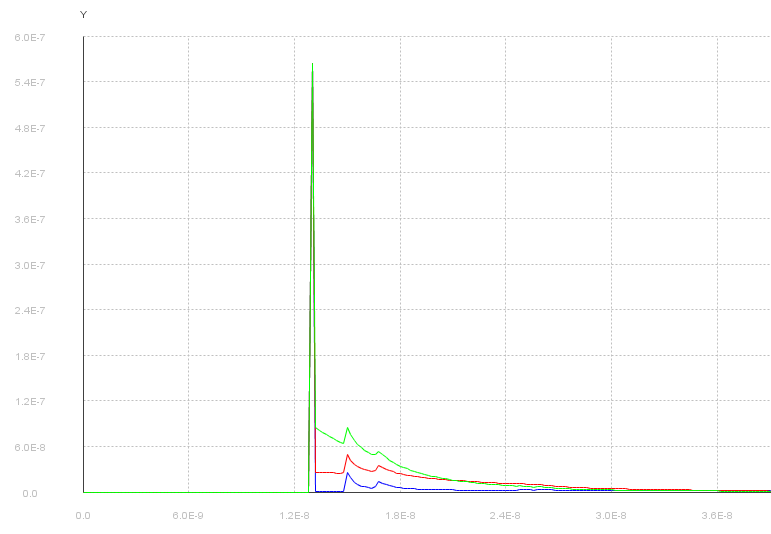
\includegraphics[width=150mm]{resultats/algo3/backward_scattering.PNG}
\caption{backward-scattering : \qquad
vert : $g = 0$ \qquad
rouge : $g = -0.5$ \qquad
bleu : $g = -0.9$}
\end{figure}

\begin{figure}[h!]
\centering
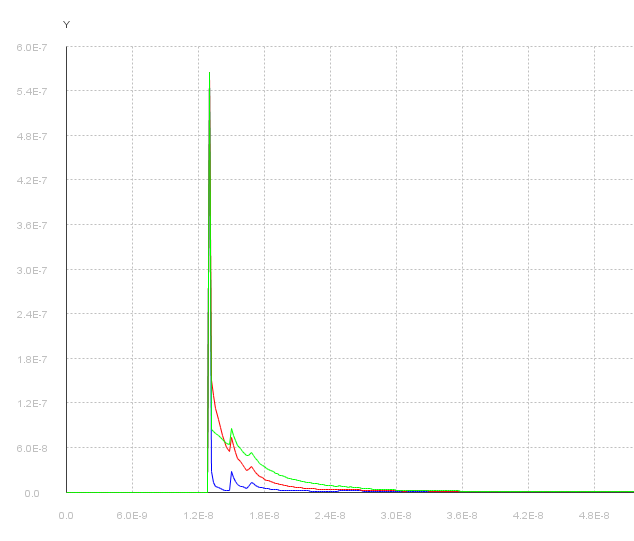
\includegraphics[width=150mm]{resultats/algo3/forward_scattering.PNG}
\caption{forward-scattering : \qquad
vert : $g = 0$ \qquad
rouge : $g = 0.5$ \qquad
bleu : $g = 0.9$}
\end{figure}
\chapter{Algorithme 4}

\section{Présentation}

Le quatrième algorithme fusionne les algo 2 et 3. Il faut effectuer deux découpes de chaque rayon, l'une pour l'in-scattering et l'autre pour le NEE. Mais la contribution de l'in-scattering en un point $p$ doit être prise en compte sur chaque point où l'on appliquera la NEE, si celui-ci est situé après le point $p$.

\section{Découpes du rayon}

Attention, pour cet algorithme il y aura besoin de deux découpes différentes : une pour appliquer l'in-scattering, l'autre pour l'out-scattering. Ces deux découpes ne créeront pas les mêmes points, mais les contributions de tous les in-scattering le long du rayon sur des points situés avant un point $p_o$ devront être prises en compte lorsqu'on y calculera l'out-scattering.
\chapter{Algorithme 5}

\section{Présentation}

Celui-ci est différent des autres. Au lieu de tirer un rayon en ligne droite et de simuler les interactions avec la fumée grâce à des coefficients d'absorption ou de dispersion, nous allons en chaque point $p_k$ (point dans le volume) estimer la probabilité de dévier dans une certaine direction. Cette approche est très semblable à l'approche actuelle (sans milieu participant) où sur chaque point surface rencontré nous tirons une nouvelle direction. Ici, régulièrement dans la fumée, nous tirons éventuellement une nouvelle direction sur la sphère complète (et non plus juste l'hémisphère). Ceci est faisable grâce à la fonction de phase, tout comme on le faisait avec la BRDF jusqu'à présent. Bien évidemment, la technique du NEE y est aussi applicable en chaque point $p_k$.

\section{Idée}

Ici, il faudra dévier le rayon à l'intérieur du milieu et plus nécessairement sur des points de surface. Pour cela, il faudra utiliser la fonction de phase, qui joue un rôle semblable à la BRDF mais pour un milieu participant. Bien évidemment, les échantillonnages de nouvelles direction ne se feront plus sur un hémisphère mais sur une sphère complète. De plus, la probabilité de dévier dépend des paramètres du milieu, de ce fait un rayon ne dévie pas régulièrement selon un pas fixé.\par
Je n'ai pas eu le temps de m'y mettre mais il serait très intéressant de créer une interface pour les fonctions de phase, tout comme il en existe déjà une pour les BRDF.


%%%%%%%%%%%%%%%%%%%%
%%% Bibliography %%%
%%%%%%%%%%%%%%%%%%%%

%\bibliographystyle{plain}
%\bibliography{bibliographie}

\end{document}